\documentclass[11pt,letterpaper]{article}
\usepackage{graphicx, geometry, amsmath, hyperref, url, natbib, booktabs, xcolor, listings}
\usepackage{xurl}
\geometry{margin=1in}
\hypersetup{colorlinks=true, linkcolor=black, citecolor=black, urlcolor=black}
\renewcommand{\topfraction}{0.9}
\renewcommand{\bottomfraction}{0.8}
\renewcommand{\textfraction}{0.07}
\renewcommand{\floatpagefraction}{0.9}
\usepackage{array}
\usepackage{tabularx}
\usepackage{longtable}
\usepackage{enumitem}
\setlist{itemsep=1pt, topsep=3pt}
\usepackage[compact]{titlesec}
\usepackage[font=small]{caption}
\makeatletter
\setlength{\@fptop}{0pt}
\setlength{\@fpsep}{12pt}
\setlength{\@fpbot}{0pt plus 1fil}
\makeatother
\setlength{\textfloatsep}{14pt plus 2pt minus 4pt}
\setlength{\emergencystretch}{1em}

% Generated tokens: \tok for a token without a leading space, \stok for one with a leading space.
\newcommand{\tok}[1]{\texttt{#1}}
\newcommand{\stok}[1]{\texttt{\textvisiblespace#1}}
\newcolumntype{L}[1]{>{\raggedright\arraybackslash}p{#1}}
\newcolumntype{Y}{>{\raggedright\arraybackslash}X}

\hypersetup{pdftitle={A single forking token fixes the algorithm a code model writes}}

\begin{document}

\begin{center}
{\LARGE A single forking token fixes the algorithm a code model writes\par}
\end{center}
\vspace{0.5em}

\begin{abstract}
Instruction-tuned code models write the same algorithm for a task almost every time, and sampling temperature is the decoding parameter usually raised to change that. We locate where in generation the algorithm is chosen, labelling programs by execution and resampling continuations from every prefix, and compare interventions under shared random seeds. A single forking token fixes the algorithm. On the three tasks on which Qwen3-8B already writes two algorithms, the algorithm's entropy given the class of that token was at most 0.189 bits (bootstrap 95\% CI 0.123 to 0.239), down from 0.82 to 1.02 bits before it: a margin of $-0.111$ bits (95\% CI $-0.177$ to $-0.061$) below the 0.3-bit bar of a preregistered test that all three tasks passed. A blind relocation found such tokens on two held-out gemma-3-4b-it tasks, but not on Llama-3.1-8B-Instruct's grid task. Temperature acts only through that token's odds: where the default leads there by several nats, no temperature from 0.3 to 1.3 changed any seed's algorithm, whereas random perturbations of the prompt's task specification states, which set those odds, changed it in 55\% of seeds on two of those tasks, across one unperturbed and three perturbed runs (difference from temperature over seeds 0.545, 95\% CI 0.41 to 0.67; preregistered). Predicting the size of the temperature effect from the logits of that token succeeded on only one of the three tasks. No decoding parameter, instruction, ban or activation edit produced a new algorithm: decoding parameters (temperature, top-$p$, min-$p$) rephrase a solution, but the idea is chosen at one token among options the model already holds.
\end{abstract}

\section{Introduction}
\label{sec:intro}

Ask an instruction-tuned code model to implement a path search and it writes BFS, that is, breadth-first search; ask for a weighted shortest path and it writes Dijkstra's algorithm. Across six independent baselines, Qwen3-8B~\citep{Yang2025} wrote BFS in 1,199 of 1,200 programs for grid path search and Dijkstra in 1,174 of 1,200 programs for shortest path. It wrote one algorithm in at least 49 of 50 programs on each of 13 further tasks derived from LeetCode, and eight more open-weight configurations wrote BFS or DFS, that is, depth-first search, on the grid task. This is a code instance of generative monoculture~\citep{Wu2024}, also reported for other models~\citep{Narula2026,Lee2025}. It matters because the algorithm fixes a program's complexity and failure modes, and a model that always writes the textbook default cannot be asked for anything else by sampling it again.

The usual remedy is to change how the model samples or what it reads: raise the sampling temperature~\citep{Peeperkorn2024}, truncate the distribution differently~\citep{Nguyen2024}, add randomness to the input~\citep{Nagarajan2025}, or forbid the techniques of earlier solutions~\citep{Lu2025}. Whether such interventions change the idea or only its wording is rarely measured, because diversity metrics score text or rely on a language-model judge~\citep{Lee2025} and independent samples confound an intervention with sampling noise. Code permits a sharper test: running two programs decides whether they implement the same algorithm, and reusing the same random numbers in every condition holds the noise fixed~\citep{Ravfogel2024}.

Judging an intervention also requires knowing where the choice is made. Resampling studies find forking tokens, positions at which resampling the continuation changes the outcome sharply~\citep{Bigelow2024}, and reinforcement learning acts mainly at a few such high-entropy positions~\citep{Wang2025,Meng2026}, but these studies concern answers to reasoning problems. Where a code model chooses the algorithm it implements has not been located.

We locate that choice token by token, labelling every program by execution and comparing interventions on identical noise. Our contributions are the following.

\begin{itemize}
\item \textbf{One forking token fixes the algorithm (Section~\ref{sec:res-fork}).} On the three mixed tasks, on which Qwen3-8B writes two algorithms, the algorithm's entropy given the class of one generated token is at most 0.189 bits (95\% CI 0.123 to 0.239), a margin of $-0.111$ bits (95\% CI $-0.177$ to $-0.061$) against a preregistered 0.3-bit bar that all three tasks passed.
\item \textbf{Temperature only reweights that token (Section~\ref{sec:res-temp}).} Where the default leads there by 4.85 to 7.46 nats, no temperature from 0.3 to 1.3 changed the algorithm of any of 20 seeds on three tasks, while phrasings multiplied; predicting the size of the temperature effect from the logits of that token worked on one of the three mixed tasks.
\item \textbf{The task specification states set its odds (Section~\ref{sec:res-states}).} Random perturbations of those states changed the algorithm in 55\% of seeds on two tasks, across one unperturbed and three perturbed runs, and patching in the states of a prompt that names the alternative wrote it on 30 of 30 seeds.
\item \textbf{Post-training widened the margin at that token (Section~\ref{sec:res-base})} by 2.11 to 13.41 nats over Qwen3-8B-Base on three collapsed tasks, on which the model writes one algorithm.
\item \textbf{No route produced a confirmed new algorithm (Sections~\ref{sec:res-prompts} and~\ref{sec:res-novel}).} Context seeds, novelty instructions and bans moved the choice only among known algorithms, and none of 45,892 audited correct programs was new; a program search with an evaluator gave eight programs one reader classed as new, which its replication did not reproduce.
\end{itemize}

Figure~\ref{fig:overview} traces the account on minimum spanning tree weight, with shortest path for the temperature margin, and Figure~\ref{fig:resampling} shows the measurement it rests on.

\begin{figure}[!htbp]
  \centering
  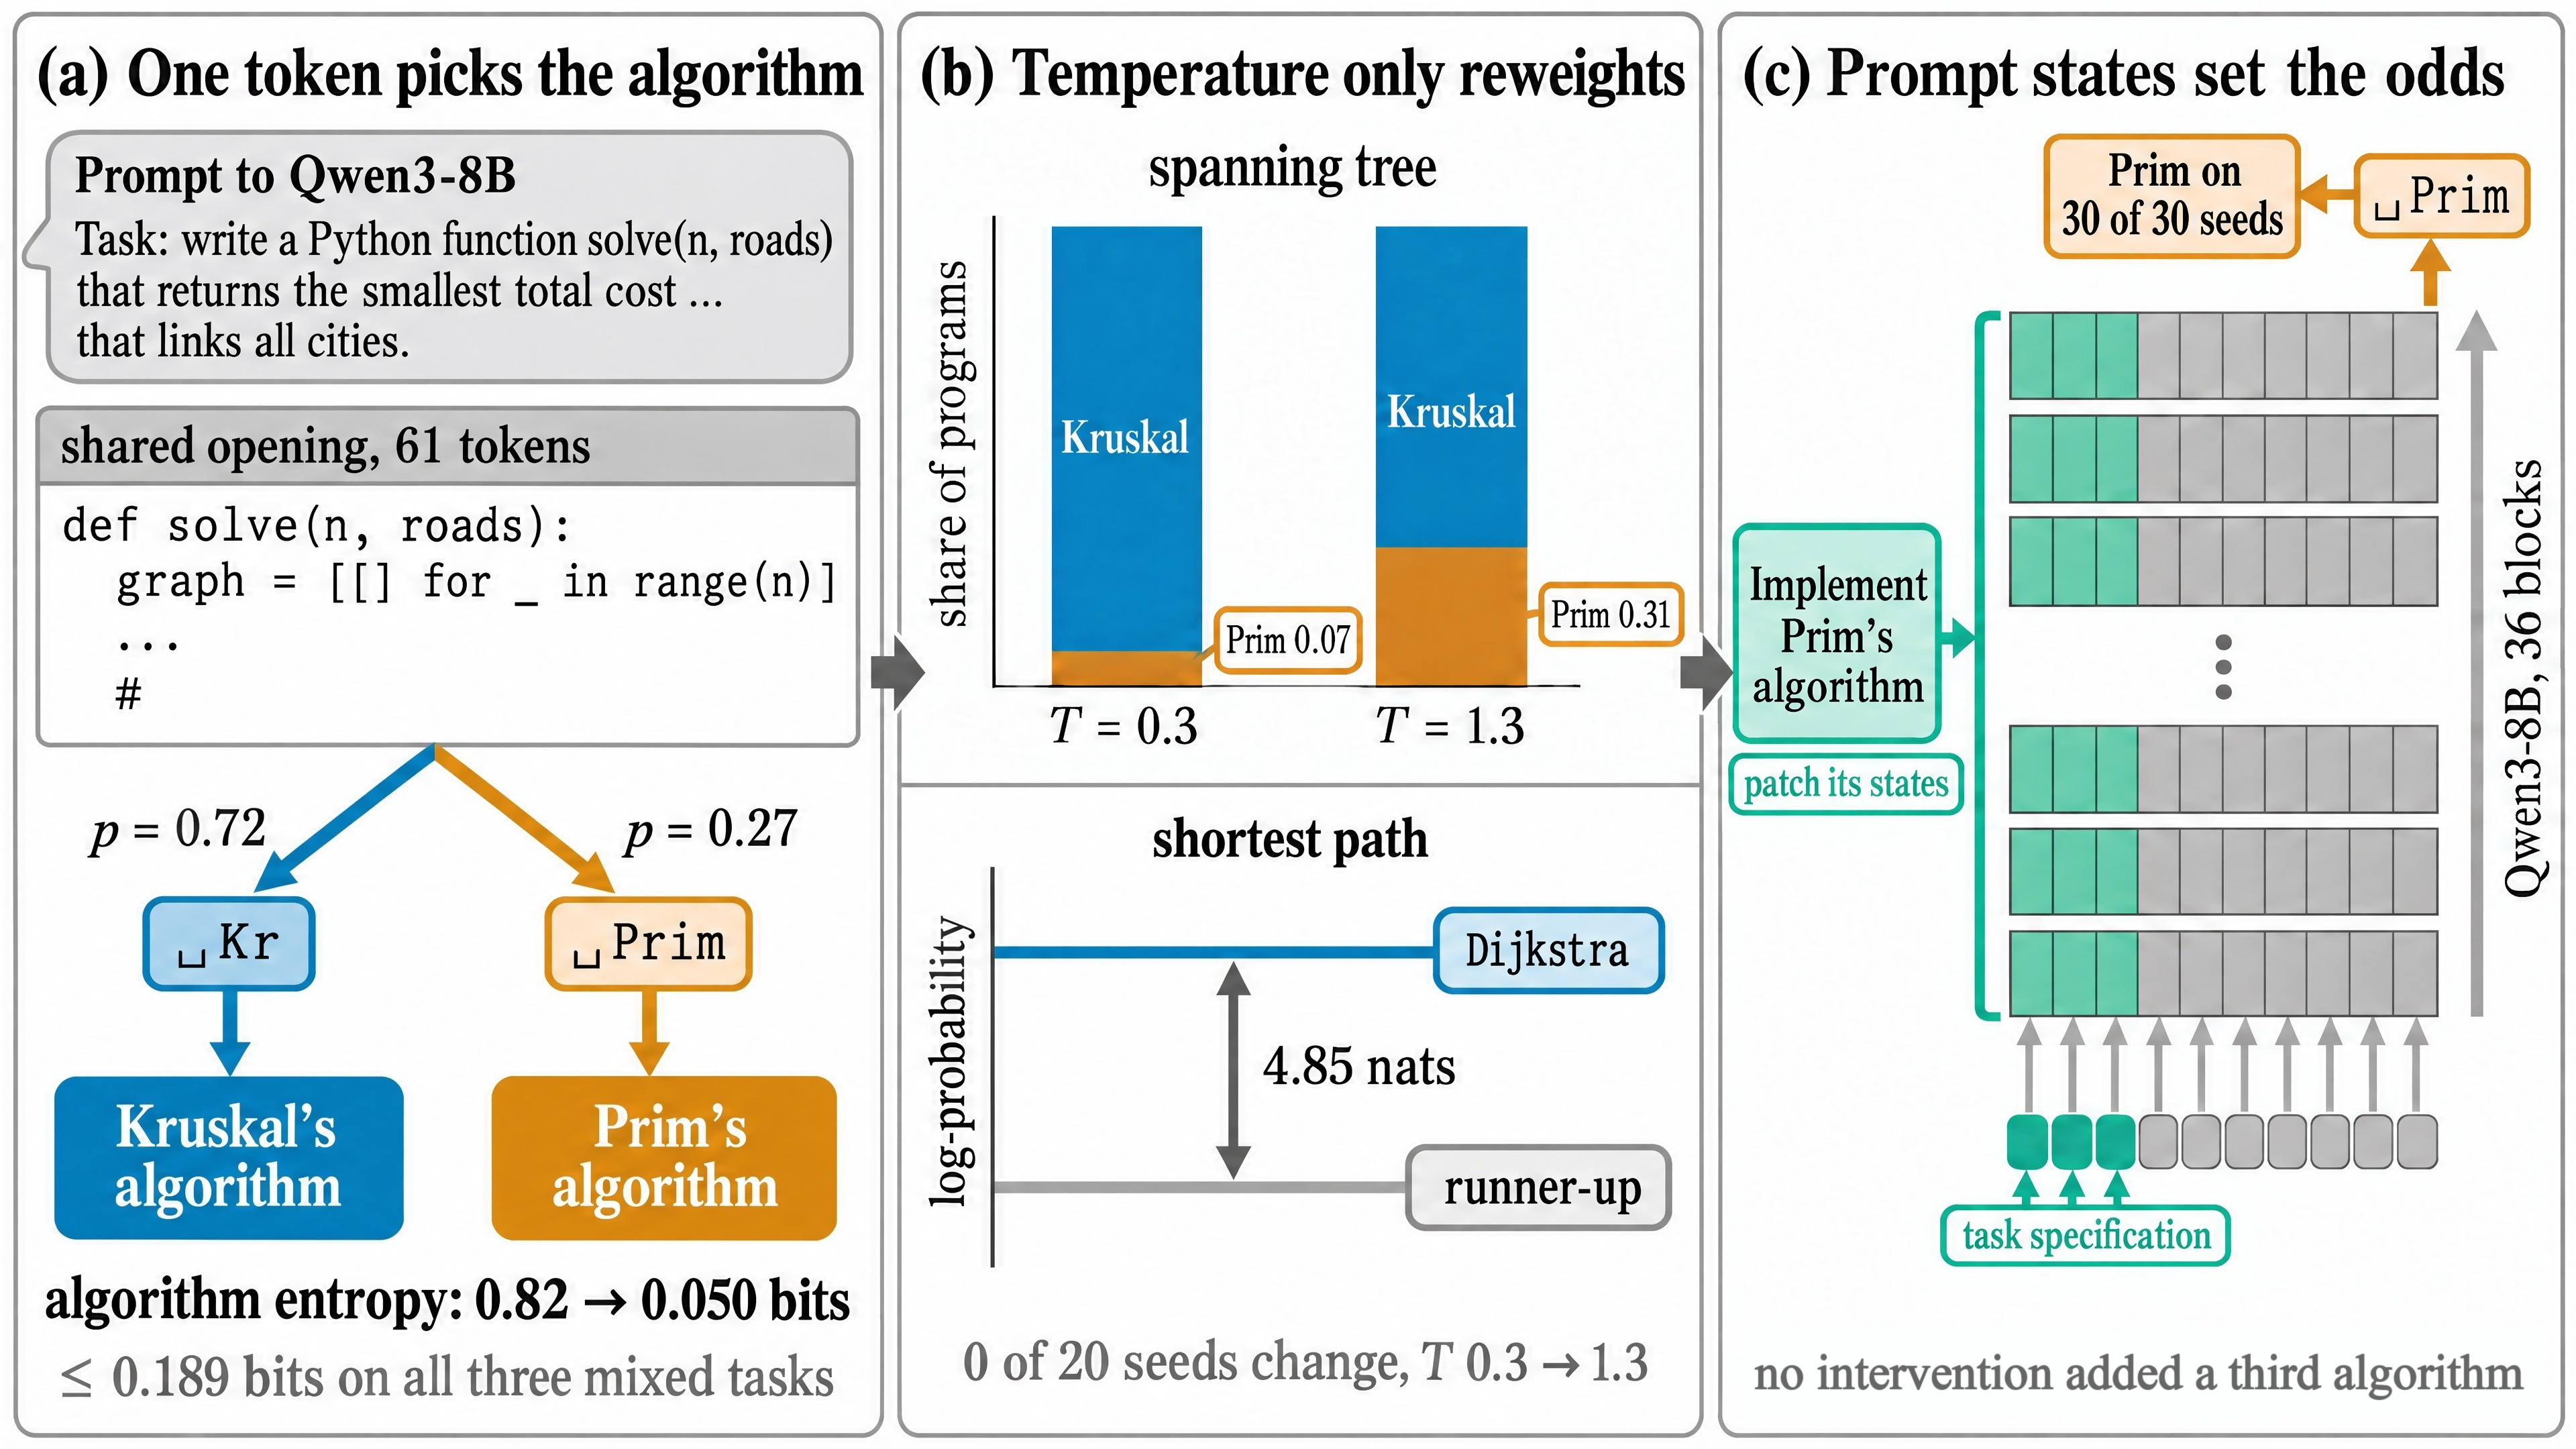
\includegraphics[width=\linewidth,height=0.45\textheight,keepaspectratio]{figures/fig1_v0.jpg}
  \caption{One forking token fixes the algorithm Qwen3-8B writes. (a) After a shared opening (grey), \stok{Kr} leads to Kruskal (blue) and \stok{Prim} to Prim (orange). (b) Temperature only reweights them; on shortest path, Dijkstra's 4.85-nat lead holds all 20 seeds. (c) Patching in task specification states (green) gives Prim on 30 of 30 seeds. Drawn overview; numbers from Section~\ref{sec:results}.}
  \label{fig:overview}
\end{figure}

\begin{figure}[!htbp]
  \centering
  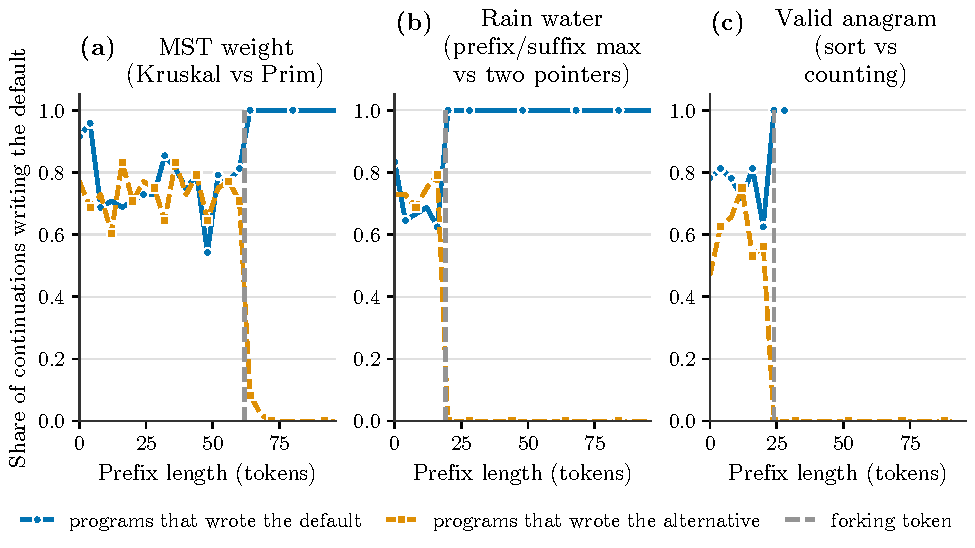
\includegraphics[width=\linewidth,height=0.45\textheight,keepaspectratio]{figures/fig2_v0.pdf}
  \caption{Prefix resampling locates a single forking token in Qwen3-8B (temperature 1) across three coding tasks. Each point is the mean, over 8 resampled continuations per program and 6 sampled programs per line (4 for valid anagram), of the share writing the task's default algorithm; both lines settle to 1 or 0 within a few tokens of the dashed forking token.}
  \label{fig:resampling}
\end{figure}

\section{Related Work}
\label{sec:related}

\paragraph{Algorithmic diversity of code models.} Generative monoculture names the narrowing of output diversity relative to what a task admits, code included~\citep{Wu2024}. \citet{Lee2025} cluster correct solutions by algorithm with a language-model judge and find low algorithmic diversity that rises with temperature above 1 at a cost in correctness; prompt cues steer the choice~\citep{Narula2026}, denial prompting forbids earlier techniques~\citep{Lu2025}, and implementation priors explain why constraints against a default fail~\citep{Tang2026}. We label the mechanism a program executes and locate where the choice is made.

\paragraph{Decoding and prompting for diversity.} Temperature correlates only weakly with novelty in stories~\citep{Peeperkorn2024}. Min-$p$ sampling~\citep{Nguyen2024}, dynamic temperature driven by entropy~\citep{Zhang2024} and adaptive temperature for code~\citep{Zhu2024} reshape the next-token distribution; seed-conditioning~\citep{Nagarajan2025}, intent factored generation~\citep{Ahmed2025} and PlanSearch~\citep{Wang2024} add randomness or plans before the answer; chat templates themselves collapse diversity~\citep{Yun2025}. We compare such interventions on shared sampling noise, as Gumbel counterfactual generation does~\citep{Ravfogel2024}.

\paragraph{Forking tokens and post-training.} Forking Paths finds tokens at which the outcome distribution of resampled continuations changes abruptly~\citep{Bigelow2024}; hidden states anticipate such outcomes~\citep{Zur2025}, and high-entropy minority tokens~\citep{Wang2025} and thought anchors~\citep{Bogdan2025} carry the decisions of reasoning traces. Reinforcement learning mostly reweights choices the base model already considers~\citep{Meng2026}, most tokens of an aligned model are the base model's top token~\citep{Lin2023}, alignment can sit in a response's first tokens~\citep{Qi2024}, aligned models are less diverse than base models~\citep{Kirk2023,West2025} and concentrate probability on fewer continuations~\citep{Yang2025a}, and in code, self-distillation separates forks that need exploration from locks that need precision~\citep{Zhang2026}. We add which algorithm follows forks in code, and the post-training margin there.

\paragraph{Activation interventions and geometry.} Steering vectors~\citep{Rimsky2024} and single directions for refusal~\citep{Arditi2024} or truth~\citep{Marks2023} edit the residual stream, activation noise and steering raise output diversity~\citep{Khalid2026,Zhu2026}, and prompt states encode attributes of the coming response~\citep{Dong2025}. Distributed alignment search (DAS) fits causal subspaces of low rank~\citep{Geiger2023,Wu2023}, but subspace patching can act through pathways the model does not use~\citep{Makelov2023}, and expressive maps can align a network with algorithms it does not implement~\citep{Sutter2025}. Sparse autoencoders~\citep{Lieberum2024} often steer worse than simple baselines~\citep{Wu2025}; manifold steering follows fitted manifolds~\citep{Wurgaft2026} measured by geodesic distances~\citep{Tenenbaum2000}. We ask which site sets the forking token's odds.

\paragraph{Program search with an evaluator.} FunSearch~\citep{RomeraParedes2023}, Evolution of Heuristics~\citep{Liu2024}, ReEvo~\citep{Ye2024} and AlphaEvolve~\citep{Novikov2025} pair a language-model proposer with an executable evaluator, and many bin packing heuristics found this way reduce to simple parametric rules~\citep{Herrmann2026}. We ask only whether selection yields new heuristics from an 8B model.

\section{Method}
\label{sec:method}

\paragraph{Labelling programs.}
Each task has a catalogue of three to ten known algorithms (Appendix~\ref{app:tasks}). A program is correct if it passes all of its task's hidden tests (40 to 48 per path task, 684 across the 13 bench tasks of Section~\ref{sec:setup}) in a sandbox with a time limit per test case. A runtime tracer of operations on data structures, grid reads, edge relaxations and recursion assigns the mechanism, rules over the abstract syntax tree assign a second label, and a blind language-model judge sees only programs on which the two disagree. The combined label agreed with adjudicated gold labels at Cohen's kappa 0.966 on the path tasks (Appendix~\ref{app:tasks}). A program matching no catalogue entry is labelled other and audited for novelty (below). For a given model, a task's default is the algorithm the model writes most often; we call the task mixed when the model writes two algorithms, each in a substantial share of programs, and collapsed when it writes one in nearly all of them.

\paragraph{Locating the forking token.}
Following Forking Paths~\citep{Bigelow2024}, prefix resampling keeps the first $j$ generated tokens (the prefix length) of programs the model sampled itself, for $j = 0, 4, 8, \ldots$, draws 8 continuations at temperature 1 from each prefix, labels them, and tracks the outcome distribution over algorithms. A Bayesian change-point model with a permutation null marks where the share of the sampled program's own algorithm jumps by at least 0.4, and 20 further continuations there and at control positions confirm it, because estimates from few samples are noisy~\citep{Bigelow2026}. We call the confirmed position the fork and the tokens before it, which the sampled programs share, the opening. At the fork we read the teacher-forced next-token distribution and group candidate tokens into classes by the algorithm that continuations forced to begin with them write. The entropy $H(A \mid C)$ of the algorithm $A$ given the class $C$ of the sampled forking token measures how much of the choice the token settles.

\paragraph{Predicting temperature's effect.}
The forking-token prediction at temperature $T$ composes the tempered probability of staying on the opening, the tempered distribution over forking tokens, and the algorithm each forking token leads to. It was committed by its hash before any sample at the target temperatures and is scored by the total variation distance between predicted and observed algorithm distributions, averaged over $T \in \{0.3, 0.7, 1.0, 1.3\}$, against a baseline that predicts no change (the $T = 1$ shares at every $T$), tempering of those shares themselves, and a variant placed at the position of highest entropy. On collapsed tasks we read the forking-token margin, the gap in log probability, in nats, between the token class of the default and the strongest alternative class.

\paragraph{Comparisons under shared seeds.}
Paired comparisons use common random numbers: each sample slot, which we call a seed, owns one stream of uniform random numbers, and the sampler maps the tempered next-token distribution to a token by inverse-CDF lookup, so two programs from one seed differ only by the condition. We count the seeds whose algorithm differs across a set of conditions, compare paired outcomes by exact McNemar tests on discordant seeds~\citep{Mcnemar1947}, and test contrasts over seeds by sign flips.

\paragraph{Perturbing and patching task specification states.}
A prompt has a condition sentence (empty, neutral or a ban, a negative constraint naming algorithms not to use), a task specification (problem statement and function signature) and a last token, from whose state the first generated token is predicted; we call the residual stream states at the tokens of the task specification its task specification states. Each ban and each instruction has a control prompt of the same length, in tokens, in which filler replaces the words that state the condition: irrelevant nouns replace the algorithm names of a ban, and filler tokens stand in place of the tokens of an instruction. Steering along a random direction, a form of activation steering~\citep{Rimsky2024}, writes a random unit direction $u$ into the residual stream during the prompt pass only. At block $l$ and position $i$ of the task specification, the component along $u$, measured from the control prompt's state, is set to $\alpha\, n_{l,i}$, where $n_{l,i}$ is the norm of the displacement that the ban sentence itself produces there. The intervention strength $\alpha$ is thus a multiple of the displacement the ban sentence produces at that site: $\alpha = 1$ is a random displacement of the size that a ban of one sentence causes. Unless stated, steering is applied at blocks 12 to 23. Activation patching replaces the task specification states of a prompt, at every block, with those of another prompt of the same length, for example \texttt{Implement Prim's algorithm} patched into its control prompt of the same length; a random replacement of matched norm serves as a baseline.

\paragraph{Diversity and novelty.}
Diversity is the effective number of algorithms among correct programs, the exponential of the Shannon entropy of their algorithm labels, that is, the Hill number of order 1~\citep{Hill1973}, rarefied to subsamples of 25. Phrasings are clusters of programs whose AST 4-gram shingles, after identifiers are normalised, reach a Jaccard similarity of 0.8. A correct program labelled other counts as novel only if, after stress tests, a comparison with its nearest known solutions by tree edit distance~\citep{Zhang1989}, two blind judges gated on known control programs and a full manual read, it implements no known algorithm; with none among $n$ programs, the rule of three bounds the rate by $3/n$.

\section{Experimental Setup}
\label{sec:setup}

\paragraph{Models.} The main model is Qwen3-8B~\citep{Yang2025} in non-thinking mode at temperature 1, in bfloat16 with exact common random numbers, and in some experiments in a W8A8 engine, with 8-bit floating-point weights and activations, on smaller GPUs; the perturbation results hold in bfloat16 (Appendix~\ref{app:controls}). We chose it as an open-weight, instruction-tuned model that runs these experiments on one GPU, with thinking and non-thinking modes and a released base model: Qwen3-8B-Base serves for the base comparison, and gemma-3-4b-it, gemma-3-4b-pt~\citep{Team2025} and Llama-3.1-8B-Instruct~\citep{Grattafiori2024} as further families. The ban experiments add Qwen3-14B and Qwen3-32B in thinking and non-thinking mode, gemma-3-27b-it and the code model Qwen2.5-Coder-32B-Instruct~\citep{Qwen2024}, so that obeying a ban can be compared across model size, thinking mode, family and code training.

\paragraph{Tasks.} The two path search tasks follow a public set of creativity probes for code models~\citep{Pesjak2026}: grid path search with moves to the four neighbouring cells, where any valid path is accepted so BFS is not forced, and weighted shortest path between one pair of nodes on a directed graph. Thirteen bench tasks derived from LeetCode problems~\citep{Xia2025}, such as $k$-th smallest element, two sum and connected components, carry 684 hidden test cases and references for 54 algorithms. Sixteen further tasks, among them minimum spanning tree weight, trapped rain water and valid anagram, were built the same way. Each task has five prompt templates. Appendix~\ref{app:tasks} gives each task group's input, expected output, tests and labelling, and Appendix~\ref{app:search} describes the online bin packing and TSP tasks of the program search.

\paragraph{Preregistration and audits.} Every decisive rule and prediction was committed by its hash, in a SHA-256 chain, before the samples it governs, every headline number was recomputed from raw rows by an independent script, and placebo versions of each test were checked to fail. Shares carry Clopper-Pearson~\citep{Clopper1934} or Wilson~\citep{Wilson1927} intervals, contrasts bootstrap intervals. Each experiment fits on one GPU, such as an RTX 4090 or an RTX 2000 Ada, in about 1 to 3 hours of GPU time, with vLLM~\citep{Kwon2023} for unpaired sampling. Code, prompts, raw generations, labels and the scripts that recompute each number are in the paper's code repository~\href{https://github.com/ai-inventor-papers/ai-invention-295f8e-prompt-bans-substitute-not-just-subtract/tree/fork/run_jSassd-YWLVC}{[code]}, and Appendix~\ref{app:code} links each result to the folder of the experiment that produced it.

\section{Results}
\label{sec:results}

\subsection{One forking token fixes the algorithm}
\label{sec:res-fork}

On the three mixed tasks of Qwen3-8B, sampled programs share an opening of 18 to 61 tokens, and the next token settles the algorithm (Figure~\ref{fig:resampling}, Table~\ref{tab:forks}): the share of continuations writing the default stays between 0.47 and 0.96 along the opening and jumps to 1 or 0 at the forking token. The preregistered test required the entropy of the algorithm given the class of the forking token to be at most 0.3 bits on at least two tasks. It passed on all three: 0.050 bits (bootstrap 95\% CI 0.014 to 0.096) on minimum spanning tree weight, 0.153 (0.091 to 0.203) on trapped rain water and 0.189 (0.123 to 0.239) on valid anagram, against 0.82, 0.97 and 1.02 bits at the fork before the token is sampled. On the least decisive task the margin to the bar is $-0.111$ bits (95\% CI $-0.177$ to $-0.061$). On minimum spanning tree weight the opening ends with a comment marker; the next token is \stok{Kr} with probability 0.72, after which every continuation writes Kruskal's algorithm, or \stok{Prim} with probability 0.27, after which 97\% write Prim's (\textvisiblespace\ marks a leading space).

\begin{table}[!htbp]
\centering
\footnotesize
\caption{Forking tokens located by prefix resampling (Qwen: Qwen3-8B; Gemma: gemma-3-4b-it; Llama: Llama-3.1-8B-Instruct). $H$: the algorithm's entropy in bits at the fork, before the token is sampled and given the sampled token's class (preregistered bar 0.3); the blind relocation used fresh samples and allows a second decision within two tokens.}
\label{tab:forks}
\begin{tabularx}{\linewidth}{@{}L{3.5cm}L{1.2cm}YL{0.9cm}L{2.1cm}L{1.5cm}@{}}
\toprule
Task (model) & Opening (tokens) & Forking token (probability) $\rightarrow$ algorithm & $H$ at fork & $H$ given token [95\% CI] & Blind\newline relocation \\
\midrule
Minimum spanning tree weight (Qwen) & 61 & \stok{Kr} (0.72) $\rightarrow$ Kruskal; \stok{Prim} (0.27) $\rightarrow$ Prim & 0.82 & 0.050 [0.014, 0.096] & 0.004 \\
Trapped rain water (Qwen) & 18 & \stok{n} $\rightarrow$ prefix/suffix maxima; \stok{left} $\rightarrow$ two pointers & 0.97 & 0.153 [0.091, 0.203] & below 0.001 \\
Valid anagram (Qwen) & 23 & \stok{return} $\rightarrow$ sort; \stok{count} $\rightarrow$ counting & 1.02 & 0.189 [0.123, 0.239] & below 0.001 (count branch) \\
Substring search (Gemma, held out) & 31 & \tok{for} (0.73) $\rightarrow$ naive scan; \tok{try} (0.10) $\rightarrow$ library call & -- & -- & 0.001 \\
First and last position (Gemma, held out) & 12 & \tok{first} (0.95) $\rightarrow$ linear scan; \tok{left} (0.05) $\rightarrow$ binary search & -- & -- & 0.001 \\
Grid path search (Gemma) & 32 & \stok{visited} $\rightarrow$ DFS; blank line, \tok{if}, \tok{queue} $\rightarrow$ BFS & -- & -- & -- \\
Grid path search (Llama, held out) & 52 & \stok{visited} (0.45) $\rightarrow$ DFS; \stok{queue} (0.25) $\rightarrow$ BFS & -- & -- & 0.629 \\
\bottomrule
\end{tabularx}
\end{table}

A blind locator on fresh samples recovered these forks (on valid anagram, the next decision inside the counting branch), found single forking tokens on two held-out gemma-3-4b-it tasks, and showed Gemma's grid task forking the same way (Table~\ref{tab:forks}); collapsed tasks have forks too, which surface in perturbed and banned samples (Appendix~\ref{app:tasks}).

The fork is not universal. On Llama-3.1-8B-Instruct's grid task the openings that reach a forking token cover about 2\% of programs, and the algorithm keeps 0.63 bits given the located decisions; on weighted shortest path, perturbed generations stay undecided for at least 60 tokens, and on $k$-th smallest the algorithm is fixed before the first generated token. Where a fork exists it is a high-entropy position (Appendix~\ref{app:tasks}).

\subsection{Temperature only reweights the forking token}
\label{sec:res-temp}

If one token decides, temperature can act on the algorithm only through that token's distribution and the probability of reaching it. Figure~\ref{fig:temperature} compares the forking-token prediction, committed before sampling, with the observed share of the minority algorithm at four temperatures on shared token streams. Lowering the temperature from 1.0 to 0.3 removed the minority algorithm in paired seeds as predicted: all 18 discordant seeds moved to the default on minimum spanning tree weight (exact McNemar $p = 3.8\times10^{-6}$), as did all 10 on Gemma's substring search and all 13 on its first and last position.

\begin{figure}[!htbp]
  \centering
  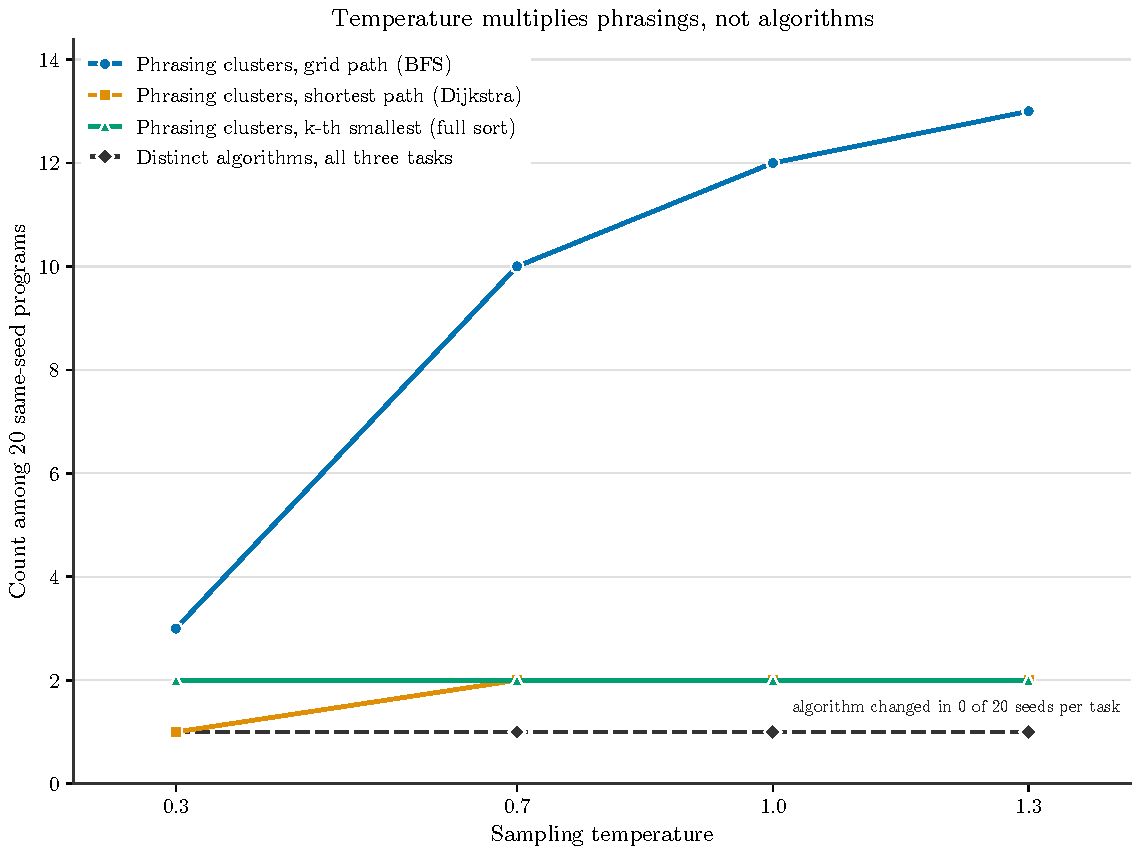
\includegraphics[width=\linewidth,height=0.45\textheight,keepaspectratio]{figures/fig3_v0.pdf}
  \caption{Lowering the sampling temperature shrinks the share of the minority algorithm roughly as the forking-token prediction implies, but the flat baseline of no change is often nearly as close to the observed points, and on the held-out Llama panel (f) the observed share diverges from both. F, B: each curve's mean total variation distance from the data. G: gemma-3-4b-it; L: Llama-3.1-8B-Instruct; others Qwen3-8B; $N = 100$ per cell.}
  \label{fig:temperature}
\end{figure}

The prediction's mean total variation distance from the observed shares (F in Figure~\ref{fig:temperature}) was 0.014 to 0.054 on five of six tasks, under the preregistered bar of 0.10, and 0.142 on Llama's grid task, whose many openings it does not model. Predicting no change (B) was almost as good: the forking-token prediction beat it on only 4 of 6 tasks (exact sign test $p = 0.34$), though it beat the two other rival predictions on 5 of 6. A simpler prediction from the forking token alone, committed before sampling on the three mixed tasks, matched the observed response only on minimum spanning tree weight, one task against the two its test required. The forking token explains the direction and mechanism of temperature's effect, but not yet its size.

On collapsed tasks the forking-token margin puts the alternative out of reach. On the control prompt of the same length the default leads the strongest alternative by 7.46 nats on grid path search, 4.85 on shortest path, 17.04 on connected components and 6.10 on $k$-th smallest. At $T = 1.3$ these margins imply rates of leaving the default of 0.002, 0.020, below 0.0001 and 0.009, and 100 continuations from each fork at $T = 1.3$ gave none. Table~\ref{tab:seeds} tests the consequence with a preregistered design on shared seeds.

\begin{table}[!htbp]
\centering
\footnotesize
\caption{Seeds (of 20) whose algorithm changes across each row's conditions under common random numbers (Qwen3-8B, non-thinking unless stated; temperatures 0.3, 0.7, 1.0 and 1.3). Counts for steering along a random direction: seeds whose algorithm differs anywhere among the unperturbed run and three perturbed runs, averaged over the 20 subsets of three among six directions. Last row: contrast with temperature over seeds, bootstrap 95\% interval.}
\label{tab:seeds}
\begin{tabularx}{\linewidth}{@{}YL{3.1cm}L{3.1cm}L{3.1cm}@{}}
\toprule
Conditions compared & Shortest path (Dijkstra) & $k$-th smallest (full sort) & Grid path (BFS) \\
\midrule
Temperature 0.3 to 1.3 (top-$p$ 1) & 0 & 0 & 0 \\
\ldots\ plus top-$k$ 10 at $T$ 0.7 & 0 & 0 & 0 \\
\ldots\ plus min-$p$ 0.1 at $T$ 2.0 & 1 & 1 & 0 \\
Thinking mode, $T$ 0.3 to 1.3 & 0 & -- & 0 of 10 \\
Random direction, $\alpha = 1$ & 17.25 & 4.55 & 2.5 \\
Random direction, $\alpha = 2$ & 19.05 & 10.6 & 8.7 \\
Contrast at $\alpha = 1$ [95\% CI] & 0.863 [0.775, 0.943] & 0.228 [0.090, 0.380] & 0.125 [0.025, 0.225] \\
\bottomrule
\end{tabularx}
\end{table}

No temperature from 0.3 to 1.3 changed the algorithm of any seed on any task (upper 95\% confidence bound on the rate per seed 0.17), in thinking mode either, although phrasings per algorithm grew with $T$ (pooled slope 0.64 per unit temperature in log phrasings at a Jaccard threshold of 0.7, 95\% CI 0.30 to 0.89). Under the same seeds, steering along a random direction at $\alpha = 1$ changed the algorithm, somewhere among the unperturbed run and three perturbed runs, for 17.25 of 20 seeds on shortest path (to Bellman-Ford or SPFA) and 4.55 on $k$-th smallest (to quickselect): a pooled contrast with temperature over seeds of 0.545 (95\% CI 0.41 to 0.67; $p = 1.0\times10^{-5}$ by sign flips). The steering's own preregistered bar of 5 seeds per task failed on $k$-th smallest, where the ban displacement that scales $\alpha$ was 0.77 times as large as in the screening experiment that selected the task (10.6 seeds at $\alpha = 2$); on shortest path it cost correctness (pass rate 0.63 against 1.00).

At a fixed seed, then, tight temperature with top-$k$ 10 yields about one idea in a few phrasings; top-$k$ 10 even gave programs identical token for token to top-$p$ 1 in 600 of 600 pairs that share a seed, since every forking token lies in the top ten. At $T = 0.3$, ten trajectories on minimum spanning tree weight were nine Kruskal programs in three phrasing clusters and one Prim program. Loosening the temperature moves mass to the second idea the forking token already weighs and multiplies phrasings (Kruskal from 4 to 22 clusters per 100-program cell between $T = 0.3$ and 1.3, Prim from 2 to 7); no third algorithm appeared.

\subsection{The task specification states set the forking token's odds}
\label{sec:res-states}

Two measurements locate what sets the forking token's distribution. The first is activation patching. Patching the task specification states of a prompt that names the minority algorithm into its control prompt of the same length wrote the minority on 30 of 30 seeds on all three mixed tasks, every patched program correct, against 7, 4 and 0 of 30 for the control prompt itself and 12, 4 and 0 for a random replacement of matched norm. It moved the teacher-forced forking-token margin by $-4.9$, $-5.5$ and $-22.1$ nats, against $-1.2$, $-2.0$ and $+0.3$ for the replacement. Patching the states of a ban of Dijkstra's algorithm into its control prompt of the same length moved 24 of 30 seeds to Bellman-Ford or SPFA (21 correct; McNemar 24:0), whereas patching the last prompt token transferred nothing on any of six tasks. On two sum and find the duplicate the ban is carried instead by the condition sentence: patching its states transferred the ban on 30 and 27 of 30 seeds, patching the task specification states on 13 and 1.

The second is steering along a random direction, whose effect depends on its site. Figure~\ref{fig:sites} counts the correct programs off the default after the same random direction, at the same strength $\alpha$ per position, is written into six sites. At the last prompt token and on the condition sentence it changed the algorithm of none of 526 and 527 correct programs, and at the task specification's late blocks (24 to 35) of only 6 of 521, and not for lack of displacement (Appendix~\ref{app:controls}). Steering the first 32 generated tokens, where the forks lie, also worked. The effects reappear in bfloat16 (Appendix~\ref{app:controls}).

\begin{figure}[!htbp]
  \centering
  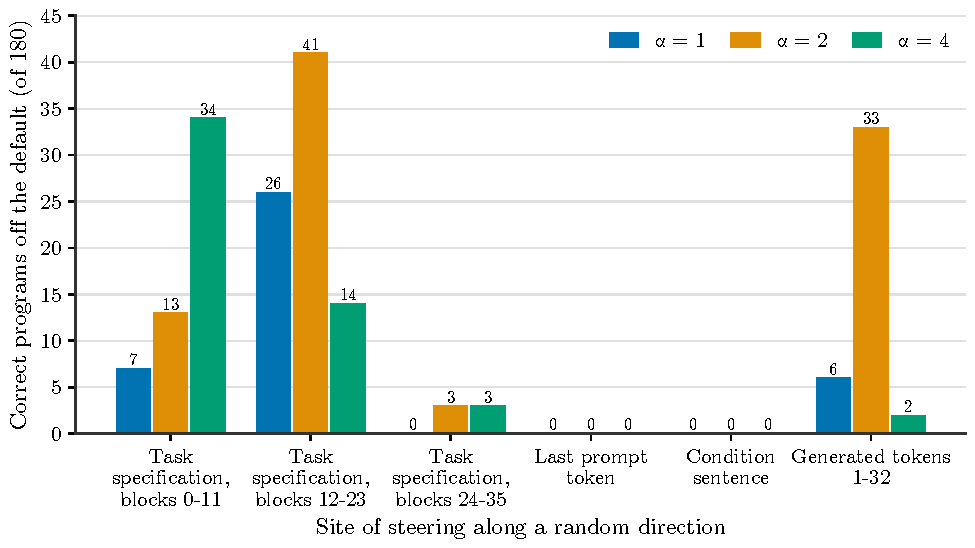
\includegraphics[width=\linewidth,height=0.45\textheight,keepaspectratio]{figures/fig4_v0.pdf}
  \caption{On Qwen3-8B (W8A8 engine), steering along a random direction changes which algorithm gets written mainly when applied to the task specification states of blocks 0--23 or to the first 32 generated tokens; steering at the last prompt token or the condition sentence never does. Bars count correct programs off the default at intervention strengths $\alpha = 1$, 2 and 4, pooled over six coding tasks (180 samples per bar); the drop at $\alpha = 4$ reflects broken programs, not reversion to the default.}
  \label{fig:sites}
\end{figure}

The perturbation reaches only known alternatives, and only on some tasks. With 40 fresh directions per task (8 on nine bench tasks), steering at $\alpha = 2$ changed the algorithm on $k$-th smallest (63\% of directions; quickselect or a size-$k$ heap), connected components (73\%; DFS or BFS), shortest path (20\%; Bellman-Ford or SPFA), two sum (13\%; brute force) and grid path (13\%; DFS), and on none of the other ten tasks. No subspace we fitted predicts which directions work (Appendix~\ref{app:controls}), and cheaper methods that act on the text reach as high an effective number of algorithms (Appendix~\ref{app:knobs}).

\subsection{Post-training widened the margin at the forking token}
\label{sec:res-base}

Is the default the base model's average answer? We scored identical token ids, formatted with the chat template, under Qwen3-8B and Qwen3-8B-Base (Appendix~\ref{app:base}). At the forking tokens of the three collapsed tasks the instruct margin exceeds the base margin by 3.27 nats on grid path search, 13.41 on connected components and 2.11 on shortest path, while the entropy at phrasing positions, which change only the wording, differs by only 0.23 to 0.31 nats, as preregistered. The default is a sharpened choice, not the base model's mean: the base model already prefers it at the fork, by 2.55 to 3.50 nats. On minimum spanning tree weight post-training even reversed the preference: mapped through the instruct model's algorithm for each token, the base model's forking-token distribution implies Prim with probability 0.68, where the instruct model writes Kruskal in 78\% of programs; Gemma's grid task shows a similar reversal. Part of this concentration reflects base-model uncertainty at the fork (Appendix~\ref{app:base}).

\subsection{Prompts move the choice among known algorithms}
\label{sec:res-prompts}

\paragraph{Context seeds and instructions.} Prepending a context seed, random words (\texttt{seed=(horse chair roof love)}) or a random string (\texttt{seed=d32qxk4nt43}), shifted the modal algorithm by at most one percentage point on both path tasks (90\% intervals within $\pm$15 points). The two long novelty instructions (\texttt{Make a fully novel algorithm never seen before}, with a 2,000-word rationale) made 84\% of 574 outputs claim a new algorithm. Yet 39\% of those contained no code, 75\% of the rest implemented catalogue algorithms, and none of the 23 correct programs outside the catalogue was new. The instructions spread the choice over known algorithms (effective numbers of algorithms 1.8 to 4.5 without thinking) at a cost in pass rate. On bin packing, \texttt{Make a new algorithm} returned best fit in 28 of 29 and 28 of 28 programs of Qwen3-14B and Qwen3-32B in thinking mode.

\paragraph{Bans.} A ban of the default is mostly obeyed and yields one known substitute: DFS on the grid task (86 of 100) and Bellman-Ford or SPFA on shortest path (83 of 100); on the bench tasks it acts where the forking tokens surface (Appendix~\ref{app:knobs}). A ban of the five grid algorithms used most is answered differently: Qwen3-8B avoided none of them and reimplemented them without their names in 41\% of programs. Across ten configurations of open-weight models, lexical compliance (no banned name in the program) exceeded mechanistic compliance (a search mechanism outside the banned set) by 0.70 (95\% CI 0.57 to 0.82), positive in all ten (descriptive; a second instrument missed its agreement threshold). Only Qwen3-32B in thinking mode obeyed often enough to clear the preregistered bar of 0.20 (17 of 50 programs correct and compliant in mechanism, that is, passing the hidden tests with a mechanism outside the banned set; Table~\ref{tab:fivename}).

\paragraph{Edge or opposite.} Figure~\ref{fig:geometry} places Qwen3-32B's baseline and ban prompts among the task specification states of forced prompts for ten grid algorithms, on the first two principal components, which hold 32.4\% and 12.0\% of the variance; the third, not shown, holds 11.0\%, so every distance below is taken in the full state space at block 31 (Appendix~\ref{app:maps}). The ban moves the prompt states from the DFS and BFS centroids, the nearest to the baseline prompts, toward other banned algorithms and leaves them farthest from Dijkstra with unit weights, although every compliant program of the obeying model that matches a catalogue algorithm is Dijkstra with unit weights (6 of 6; 9 of 9 on held-out templates). Whether Dijkstra with unit weights lies at the edge of the banned five or opposite them depends on the map. On an Isomap graph~\citep{Tenenbaum2000}, a k-nearest-neighbour graph ($k = 15$) of the full states whose geodesic distances classical multidimensional scaling embeds, its geodesic distance from the banned five is 1.63 times the median of the algorithms outside the banned set on a manifold built from prompts that name the algorithm (opposite) but 0.67 on one built from programs with the names removed (edge; Appendix~\ref{app:maps}). The geometry is correlational: steering prompt states toward the centroids of the compliant algorithms produced BFS in all 300 programs, and no manifold showed a ring.

\begin{figure}[!htbp]
  \centering
  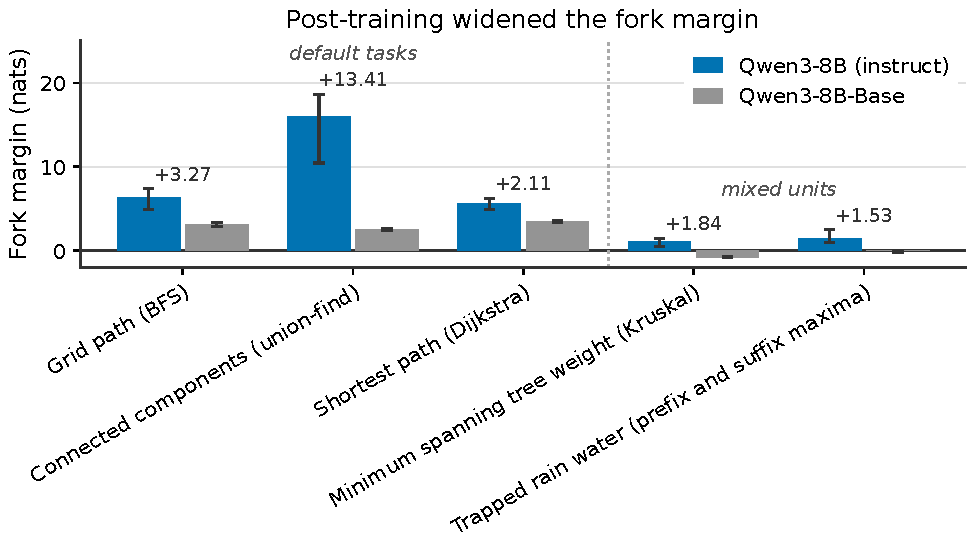
\includegraphics[width=\linewidth,height=0.45\textheight,keepaspectratio]{figures/fig5_v0.pdf}
  \caption{Under the ban, Qwen3-32B's prompt states move from the BFS and DFS centroids toward other banned algorithms, not toward Dijkstra with unit weights, the only catalogue algorithm its compliant programs use. Task specification states at block 31 on the first two principal components (the third, 11.0\% of the variance, is omitted); circles are centroids of 300 forced prompts, their area the number of programs (of 50) under the ban (labels: baseline $\rightarrow$ ban counts).}
  \label{fig:geometry}
\end{figure}

\subsection{No route produced a confirmed new algorithm}
\label{sec:res-novel}

In the nine experiments whose audits cover all of their correct programs, none of 45,892 correct programs implemented a new algorithm (bound by the rule of three 0.007\% per program); the 39 correct programs labelled other were labeller misses, catalogue variants or degenerate (Table~\ref{tab:novelty} in Appendix~\ref{app:novelty}). An evaluator helps only in part: with selection, an island-model search with Qwen3-8B as mutator beat best fit on held-out bin packing instances (1.40\% to 2.42\% excess bins on a Weibull test set, against 3.98\%), and an independent implementation reproduced the gain for three of five search variants. None beat the strongest published heuristics. One reader classed eight programs of the first search, all preferring a leftover that is a whole multiple of the item size, as a new idea, but only one of three judge families passed its control gate, short of the preregistered two, and the replication found none of its 40 audited candidates new (Appendix~\ref{app:search}).

\section{Discussion and Limitations}
\label{sec:discussion}

One forking token accounts for these results. Read this way, a code model's creativity in choosing an algorithm is the entropy of one token over a few known options, and every intervention we tested only moves mass among them. The data reject the view that the model returns the mean of its possible answers and that only context moves it elsewhere: the default is a sharpened, sometimes reversed, base-model choice, and context moved the algorithm only by changing the states that set the token's odds. Consistent with \citet{Lee2025}, temperature above 1 raised the effective number of algorithms modestly on mixed tasks, not on collapsed ones (Appendix~\ref{app:knobs}).

For practice, this suggests acting on the forking token's inputs rather than on global temperature; for evaluation, it argues for labels assigned by execution and for designs with shared seeds, without which rewritten code looks like a new idea. Internal readouts locate the decision but certify no variable for it (Appendix~\ref{app:readouts}), as \citet{Makelov2023} and \citet{Sutter2025} warn.

\subsection{Limitations}
\label{sec:limitations}

The main model is Qwen3-8B in non-thinking mode, and the account does not cover every model or task: Llama-3.1-8B-Instruct reaches its grid choice through many openings, shortest path decides late and $k$-th smallest before generation. Forks can be located by resampling only where the model already writes two algorithms; on collapsed tasks they were found in perturbed or banned samples, with margins from teacher forcing. The forking-token prediction of temperature's effect is not established as better than predicting no change, and only three held-out tasks were scored, one fewer than preregistered. Newer open-weight generations, Qwen3.5 and later, were not tested, so the forking-token, temperature, ban and geometry results need replication there.

The preregistered contrast with shared seeds ran in a W8A8 engine on two tasks that an earlier screening experiment had selected because steering along a random direction moved them; it was not rerun in bfloat16, although effects under 40 other directions reproduced there, and the perturbation moves the algorithm on only 5 of 15 tasks. The tasks are well-known problems with small catalogues of textbook algorithms the models have likely memorised, so open-ended design problems may behave differently. Two instruments missed their preset agreement thresholds, so the results for context seeds and the compliance values are descriptive. The novelty audits rest on catalogue labels for most programs and on one reader's manual reads for disputed ones, judge agreement was often low, and the program searches used at most 2,000 calls per search variant and seed, far fewer than published discovery systems. The internal sites we edited are not specific causal variables, and the geometry of Section~\ref{sec:res-prompts} is correlational and drawn only on the first two principal components; no view of three or more components was made, although every distance we report is taken in the full state space.

\section{Conclusion}
\label{sec:conclusion}

Where it could be located, the algorithm an open-weight code model writes was chosen at one sampled token, among options the model already holds. Making a model creative in this sense means placing a new option at that token, which no intervention we tested did. Future work should test the account on more model families and on tasks without a textbook catalogue, predict the size of temperature's effect from openings summed over many paths, and give program-search operators that act on the forking token's inputs.

\bibliographystyle{plainnat}
\bibliography{references}

\clearpage
\appendix

\section{Tasks, catalogues and labeller validation}
\label{app:tasks}

Every task asks for one Python function named \texttt{solve}. The paragraphs below give, for each group of tasks that share a format, what the model receives, what it must return, when a program counts as correct and how its algorithm is labelled; Table~\ref{tab:catalogues} lists the default each model writes and the catalogue against which programs are labelled. Every program runs in a sandbox against hidden tests with a time limit per test case and is correct only if it passes every test. Labels come from a runtime tracer and rules over the abstract syntax tree, and a blind language-model judge sees only programs on which the two disagree.

\paragraph{Prompts.} A prompt is an optional condition sentence and a blank line, then the task description, another blank line and one format line shared by all tasks. The description states the function signature, the input bounds and the value to return; bench tasks add a worked example. The baseline prompt of trapped rain water, a bench task without a condition sentence, reads in full:
\begin{lstlisting}[basicstyle=\footnotesize\ttfamily, breaklines=true, columns=fullflexible, keepspaces=true, upquote=true, frame=single, xleftmargin=4pt, xrightmargin=4pt]
Task: write a Python function solve(height) that returns the total amount of rain water held by a row of bars after rain. The argument height is a list of integers with 1 <= len(height) <= 20000 and 0 <= height[i] <= 100000; bar i has width 1 and height height[i], and water rests above a bar only where taller bars on both sides hold it in, never spilling past the ends of the row. For height = [0, 1, 0, 2, 1, 0, 1, 3, 2, 1, 2, 1] the answer is 6.

Use only the Python standard library. Return only one ```python code block containing the function solve and any helpers, with no example usage and no explanation.
\end{lstlisting}
On the path tasks a ban puts a sentence from templates such as \texttt{Do not use \char123 X\char125.} before the description, and a forced prompt, which names the algorithm to implement, one such as \texttt{Implement \char123 X\char125\ for this task.}, where X is the algorithm's name; the templates vary these wordings.

\paragraph{Path search tasks.} Grid path search asks for \texttt{solve(grid, start, goal)}: the grid has 1 to 30 rows and columns, given as strings in which \texttt{.} is a free cell and \texttt{\#} a wall, and start and goal are cells. A test passes if the returned list of cells runs from start to goal through free cells, each step to an orthogonal neighbour; any valid path passes, not only a shortest one, and \texttt{[]} is required when no path exists or an endpoint is a wall. Weighted shortest path asks for \texttt{solve(n, edges, s, t)} on up to 100 nodes and 600 directed edges \texttt{(u, v, w)} with weights 0 to 100; a test passes if the returned int equals the minimum total weight from \texttt{s} to \texttt{t}, with 0 when \texttt{s} equals \texttt{t} and $-1$ when \texttt{t} is unreachable. The time limit per test case is the larger of 1\,s and ten times the slowest catalogue reference on that case. The tracer labels a grid program by the order of its queue, stack and heap operations and grid reads, and a shortest path program by its edge relaxations and heap operations.

\paragraph{Bench tasks.} The 13 bench tasks are derived from LeetCode problems~\citep{Xia2025}; $k$-th smallest, for example, asks for \texttt{solve(nums, k)}. Each description gives the input bounds and a worked example, and a task-specific checker compares the answer with the expected one, ignoring order where the description fixes none. Each catalogue entry is defined by a one-line mechanism rather than a name, for example quickselect: \emph{partition around a pivot and recurse or loop into only the side that contains rank k}; runtime and syntax rules are written per task from these mechanisms.

\paragraph{Further tasks.} The 16 further tasks share the bench format; minimum spanning tree weight, for example, asks for \texttt{solve(n, roads)}. Their tests are LeetCode cases plus generated cases, and their rules were checked on references for every catalogue entry and on mutants that must fail. A program that matches no catalogue entry is labelled other and audited for novelty (Section~\ref{sec:method}).

\begin{table}[!htbp]
\centering
\footnotesize
\caption{Tasks, defaults and catalogues (Qwen3-8B unless stated).}
\label{tab:catalogues}
\begin{tabularx}{\linewidth}{@{}L{3.4cm}L{3.6cm}Y@{}}
\toprule
Task & Default & Catalogue \\
\midrule
Grid path search & BFS (gemma-3-4b-it: DFS 70\%) & BFS, DFS, iterative deepening DFS, A*, greedy best first search, bidirectional BFS, Dijkstra with unit weights, IDA*, jump point search, bidirectional A* \\
Weighted shortest path & Dijkstra & Dijkstra, Bellman-Ford or SPFA, bidirectional Dijkstra, Floyd-Warshall, Dial \\
$k$-th smallest element & full sort & full sort, size-$k$ heap, heapify and pop, quickselect, median of medians, counting sort \\
Substring search & naive scan (gemma-3-4b-it also) & naive scan, KMP, Rabin--Karp, Z algorithm, Boyer--Moore--Horspool, library find \\
Two sum & hash map & hash map, sort and two pointers, brute force, sort and binary search \\
Find the duplicate & hash set & hash set, sort and compare neighbours, Floyd cycle detection, binary search on values, index marking \\
Connected components & union--find & BFS, DFS, union--find, label propagation \\
First and last position & binary search (gemma-3-4b-it: linear scan) & binary search, bisect module, exponential search (gemma-3-4b-it adds linear scan) \\
Minimum spanning tree weight & Kruskal (0.80) & Kruskal, Prim with a heap, Prim with an array scan, Bor\r{u}vka \\
Trapped rain water & prefix and suffix maxima (0.68) & two pointers, prefix and suffix maxima, monotonic stack, split at the highest bar \\
Valid anagram & sort and compare (0.77) & sort and compare, hash map of counts, fixed 26-slot count array \\
\bottomrule
\end{tabularx}
\end{table}

\paragraph{Labeller validation.} Every labeller was checked before use on reference implementations of every catalogue algorithm and on mutated programs that must fail the hidden tests. On the path tasks the runtime tracer and the syntax rules each labelled 22 of 22 references correctly; on evaluation gold sets runtime and syntax labels agreed at kappa 0.753, the runtime label agreed with adjudication at 0.843 and the combined label at 0.966 (the runtime label missed the accuracy targets of that first gate, so every disagreement between the two labels went to the blind judge). On the 13 bench tasks all 54 references passed at no more than a quarter of their time limits, 39 mutants failed, runtime and syntax labels agreed at kappa 0.84 to 1.00, and the runtime label agreed with adjudication at 0.91 or more. Repeated style checks, in which two blind judges label 30 programs per task, agreed with the frozen labellers on 30 of 30 programs for each of the three mixed tasks. Two instruments did not pass their gates and their results are reported as descriptive: the labeller of the screening experiment on context seeds and temperature (gold agreement 93\% and 70\% on the two path tasks) and the expansion-order tracer used for bans, which reads no names (182 of 260 gold programs, against a bar of 90\%).

\paragraph{Forking tokens.} On Qwen3-8B's connected components, a collapsed task, the fork appears in perturbed and banned samples: after \stok{def} the token \stok{dfs} writes DFS and \stok{find} union--find, and forcing \stok{def\textvisiblespace dfs} after the control prompt of the same length gives correct DFS on 30 of 30 seeds. In the forking-token experiments, resampling with no prefix kept reproduced each mixed task's baseline minority share (Fisher $p$ 0.19 to 0.58). A second, blind locator repeats the forking-token procedure on fresh samples and allows a second decision within the next two tokens; on Gemma's grid task, BFS follows \stok{visited} in 1.1\% of 1,409 continuations and the other forking tokens in 95\% to 100\%. A fork lies above the 90th percentile of per-token entropy in all 209 samples that reach it, though it is not always the single position of highest entropy. On trapped rain water \stok{n} leads to prefix and suffix maximum arrays and \stok{left} to two pointers; on valid anagram \stok{return} leads to sorting and \stok{count} to counting (Table~\ref{tab:forks}).

\section{Further perturbation and patching results}
\label{app:controls}

\paragraph{Engine precision.} When 40 fixed directions were re-run at the same absolute strength in bfloat16, connected components changed algorithm under 26 of them, against 29 in the W8A8 engine, and shortest path under 6 against 8, with Spearman correlations across directions of 0.96 and 0.87 and the same substitute algorithms. A bfloat16 rerun of the site comparison of Figure~\ref{fig:sites} found the same order on $k$-th smallest (24:5 paired changes; Mantel-Haenszel odds ratio at matched displacement 4.6, 95\% CI 1.9 to 11.3), although its preregistered decision rule for comparing sites was withdrawn because steering at the condition sentence lacked common support.

\paragraph{Scale of the intervention strength.} The strength $\alpha$ must be measured against the ban displacement of Section~\ref{sec:method}, the absolute scale. Set instead as a fixed fraction of the control prompt's residual norm, a relative scale, it moved connected components to a correct alternative in 1 of 50 seeds where the absolute scale did so in 25 of 50, and in a crossed design the choice of scale accounted for a risk difference of 0.45 (95\% CI 0.35 to 0.55) against 0.03 for the direction seeds. Early blocks (0 to 11) moved 34 programs at $\alpha = 4$ in Figure~\ref{fig:sites}, but there $\alpha = 1$ is a smaller fraction of the residual norm (4.5\% to 7.2\% against 12.7\% to 18.3\% for blocks 12 to 23), so early and middle blocks are not separated.

\paragraph{Displacement at each site.} Steering at the last prompt token displaces the final state as much as steering at the task specification (median norm 141 against 159), and at matched displacement the task specification keeps an advantage in log odds of 2.15 (95\% CI 1.79 to 2.51).

\paragraph{Heterogeneity and specificity.} Single directions changed 3 to 17 of 20 seeds on shortest path and 0 to 7 on $k$-th smallest in the preregistered contrast of Table~\ref{tab:seeds}. Which directions work is reproducible across templates but not predicted by their projection on a subspace fitted to prompts that force an algorithm (pooled Spearman 0.03), and clamping a DAS subspace fitted at these states removed none of 218 algorithm changes.

\paragraph{Patching on shortest path.} The patch from \texttt{Implement Bellman-Ford or SPFA for this task} into its control prompt of the same length gave Bellman-Ford or SPFA on 30 of 30 seeds.

\section{Further intervention and ban results}
\label{app:knobs}

\begin{table}[!htbp]
\centering
\footnotesize
\caption{Highest effective number of algorithms reachable within 5 points of pass rate, by method and task (Qwen3-8B, bfloat16, common random numbers, $N = 50$ per cell). Its first row, steering along a random direction, uses the relative scale of Appendix~\ref{app:controls}, which is weaker than the absolute scale; at the absolute scale it reaches 3.22, 2.13, 1.21, 1.10 and 1.39.}
\label{tab:knobs}
\begin{tabularx}{\linewidth}{@{}Yccccc@{}}
\toprule
Method & $k$-th smallest & Connected components & Shortest path & Two sum & Grid path \\
\midrule
Activation steering, random direction & 1.98 & 1.09 & 1.18 & 1.17 & 1.06 \\
Intent factored generation, intent hot, code cool & 1.19 & 1.96 & 1.00 & 1.00 & 1.00 \\
Plan search before code & 1.09 & 1.50 & 1.07 & 1.00 & 1.00 \\
Enumerate algorithms, pick one at random & 1.83 & 1.88 & 1.24 & 1.27 & 1.08 \\
Base-model intent sentence & 1.73 & 2.53 & 1.45 & 1.61 & 1.04 \\
Temperature on tokens 1 to 32, matched in KL & 1.10 & 1.25 & 1.09 & 1.00 & 1.00 \\
\bottomrule
\end{tabularx}
\end{table}

An intent sentence written by Qwen3-8B-Base for the instruct model to implement reached a higher effective number of algorithms than steering along a random direction on three of five tasks (Table~\ref{tab:knobs}), against the preregistered prediction that steering along a random direction would match the best of the methods that act on the text. Temperature 1.3 and top-$k$ 10 reached at most 1.09 on every task, whereas temperature above 1 raised the effective number of algorithms on minimum spanning tree weight, a mixed task, from 1.82 to 2.07. In Figure~\ref{fig:temperature} the minority share barely grows above $T = 1$ on the Qwen3-8B tasks, because samples that leave the opening mostly return to the default. At $\alpha = 2$ on the relative scale the steering moved the algorithm on 19 seeds that the temperature matched to its departure did not, and the reverse on 3 (exact $p = 0.0009$), 13 of the 19 on $k$-th smallest. Raising the temperature only at the forking token raised the effective number of algorithms on valid anagram from 1.78 to 2.78 at a cost of 2 points of pass rate, but reached DFS on the collapsed connected components in only 3 to 9 of 50 programs. In thinking mode a repeat with the same seed differed at the byte level in all 20 shortest path traces yet kept every label, and adding top-$k$ 10 changed none of 20 seeds. A short story implying an approach without naming it moved shortest path toward Bellman-Ford by 66 points in the screening experiment whose labeller missed its agreement threshold and in 15 of 50 programs in one bfloat16 run, but left Dijkstra in 30 of 30 programs in another.

\paragraph{Single bans.} On the bench tasks a single ban is enforced where the forking tokens surface: forcing the default's opening up to its first body token undid the ban in 98\% to 100\% of samples, while a neutral function signature undid none. Over the 12 bench tasks, the template of a single ban was the strongest predictor of whether it was obeyed (likelihood ratio statistic 374 on 4 degrees of freedom; a placebo with shuffled templates gave $p$ 0.39), and the template \texttt{X is not allowed here.} failed on 10 of 12 tasks.

\begin{table}[!htbp]
\centering
\footnotesize
\caption{The grid ban of five names across ten open-weight configurations. Each configuration's banned set was its own five algorithms used most, which was BFS, DFS, iterative deepening DFS, A* and greedy best first search for all ten. A program is correct and compliant when it passes the hidden tests and uses a mechanism outside the banned set.}
\label{tab:fivename}
\begin{tabularx}{\linewidth}{@{}YL{3.9cm}L{1.8cm}L{2.4cm}L{1.8cm}@{}}
\toprule
Configuration & Baseline programs & Correct and compliant & Share [Wilson 95\%] & Share with a banned mechanism \\
\midrule
Qwen3-8B, thinking & BFS 30 of 30 & 0 of 30 & 0.00 [0.00, 0.11] & 1.00 \\
Qwen3-8B, non-thinking & BFS 100 of 100 & 0 of 100 & 0.00 [0.00, 0.04] & 1.00 \\
Llama-3.1-8B-Instruct & BFS 77, DFS 20, other 3 & 0 of 50 & 0.00 [0.00, 0.07] & 0.90 \\
Qwen3-14B, non-thinking & BFS 94, DFS 6 & 0 of 50 & 0.00 [0.00, 0.07] & 1.00 \\
Qwen3-14B, thinking & BFS 96, DFS 4 & 7 of 50 & 0.14 [0.07, 0.26] & 0.76 \\
Qwen3-32B, non-thinking & BFS 81, DFS 19 & 4 of 50 & 0.08 [0.03, 0.19] & 0.82 \\
Qwen3-32B, thinking & BFS 91, invalid 9 & 17 of 50 & 0.34 [0.22, 0.48] & 0.22 \\
gemma-3-27b-it & BFS 99 of 99 & 0 of 50 & 0.00 [0.00, 0.07] & 1.00 \\
Qwen2.5-Coder-32B-Instruct & DFS 52, BFS 48 & 0 of 50 & 0.00 [0.00, 0.07] & 0.94 \\
gemma-3-4b-it & DFS 70\% (separate run) & 0 of 50 & 0.00 [0.00, 0.07] & 1.00 \\
\bottomrule
\end{tabularx}
\end{table}

\paragraph{Bans of five names.} Under the ban of five names Qwen3-8B wrote BFS in 63 and DFS in 36 of 100 programs. Among programs that used a banned mechanism, 55\% to 100\% contained no alias of any banned algorithm. Qwen3-32B with thinking complied through Dijkstra with unit weights (6), Bellman-Ford or SPFA run on the grid (7), frontier search with random priorities (2), a random walk (1) and wavefront propagation (1), and its mean reasoning length rose from 6,864 to 9,090 tokens under the ban; on held-out templates 21 of its 50 programs were correct and compliant. The expansion-order tracer, which reads no names, puts the gap between lexical and mechanistic compliance at 0.61 (95\% CI 0.45 to 0.76). With an exact behavioural instrument on bin packing, renaming appeared without thinking (Qwen3-8B, gap 0.40, 95\% CI 0.21 to 0.55, but 0.08 on held-out templates) and not with it ($+0.04$ and $-0.13$ for Qwen3-14B and Qwen3-32B).

\paragraph{Bans under different instruments.} Under cumulative bans of one to five grid algorithms with thinking on, the share of programs that left the banned mechanisms at five names depends on the instrument: for Qwen3-32B it is 0.22 by the runtime label, 0.59 by hand reads of 46 programs, 0.67 by the expansion-order tracer and 0.74 by its fine classes; Qwen3-14B's compliance gap exceeds 0.4 under every reading except the fine tracer on held-out templates. Thinking traces name the banned rule in every bin packing cell, and Qwen3-32B with thinking moved to first fit in 14 of 30 programs under a best-fit ban.

\section{Base and instruct models at the forking token}
\label{app:base}

Table~\ref{tab:base} gives the margins behind Section~\ref{sec:res-base}, scored at the forks and at 64 phrasing positions of 20 programs per task. Its instruct margins come from 20 programs per task over five templates, so they differ from the margins of Section~\ref{sec:res-temp}, which were read on the control prompt of the same length. The Jensen-Shannon divergence between the two models, that is, the mean KL divergence of each from their average, is 7 to 12 times larger at the forking token than at phrasing positions on the collapsed tasks.

\begin{table}[!htbp]
\centering
\footnotesize
\caption{Forking-token margins (nats, default minus strongest alternative) of Qwen3-8B and Qwen3-8B-Base on the same token ids, the entropy change at phrasing positions, and the Jensen-Shannon divergence between the two models at the fork, at phrasing positions and at positions matched for the entropy of the base model.}
\label{tab:base}
\begin{tabularx}{\linewidth}{@{}YL{1.3cm}L{1.2cm}L{0.9cm}L{3.1cm}L{3.0cm}@{}}
\toprule
Task & Instruct margin & Base margin & Gain & Phrasing entropy change [95\% CI] & Divergence: fork / phrasing / matched \\
\midrule
Grid path search & 6.33 & 3.07 & 3.27 & 0.310 [0.292, 0.326] & 0.507 / 0.053 / 0.274 \\
Connected components & 15.96 & 2.55 & 13.41 & 0.275 [0.269, 0.282] & 0.306 / 0.042 / 0.203 \\
Weighted shortest path & 5.61 & 3.50 & 2.11 & 0.229 [0.223, 0.235] & 0.440 / 0.037 / 0.286 \\
Minimum spanning tree weight & 1.04 & $-0.80$ & 1.84 & 0.337 [0.326, 0.350] & 0.342 / 0.051 / 0.340 \\
Trapped rain water & 1.50 & $-0.03$ & 1.53 & 0.210 [0.200, 0.220] & 0.111 / 0.028 / 0.201 \\
\bottomrule
\end{tabularx}
\end{table}

On Gemma's grid task the base model puts 0.089 of the fork's mass on the DFS tokens against 0.671 for the instruct model, and the two disagree on the most likely forking token for 20 of 20 prompts. The divergence at the fork is 0.55 to 1.85 times that at positions matched for base entropy in Qwen3-8B, and 0.75 to 1.18 times in Gemma. In the weights, restoring the base unembedding rows of the three forking-token classes of connected components closes 0.548 (95\% CI 0.44 to 0.71) of the margin gap, against a median of 0.044 for isotropic edits of equal norm, almost all through the alternatives' rows (0.489) rather than the default's (0.060): post-training suppressed the readout of \stok{dfs} and \stok{bfs} more than it boosted \stok{find}. Random edits of equal norm in the residual stream's top 64 principal directions close as much ($p = 0.37$), so the effect lies in the readout but is not specific to these tokens. In generation the edit gave correct DFS in only 5 of 30 seeds, short of the preregistered 10.

\section{Manifold maps of the ban of five names}
\label{app:maps}

Table~\ref{tab:geodesic} gives the position of Dijkstra with unit weights, the only catalogue algorithm among compliant programs under the ban, on four maps. Every distance in this appendix and in Section~\ref{sec:res-prompts} is taken in the full state space: geodesic distances on a k-nearest-neighbour graph ($k = 15$) and Euclidean distances to centroids. Figure~\ref{fig:geometry} shows the first map on its first two principal components, which hold 32.4\% and 12.0\% of the variance; the third, not shown, holds 11.0\%. The states of the individual prompts were not kept with the published results, so a view of the first three components could not be drawn afterwards. In the full state space the baseline prompt states lie nearest the DFS and BFS centroids (mean Euclidean distances 7.35 and 7.40), and the ban prompt states lie nearest iterative deepening DFS and greedy best first search (8.64 and 8.72) and farthest from Dijkstra with unit weights (11.14, the farthest of the ten centroids, as for the held-out ban prompts). On the map built from prompts that name the algorithm, the Euclidean distance of the centroid of Dijkstra with unit weights from the banned five, 6.66 against a median of 5.60, agrees with its geodesic ratio. The preregistered prediction of opposite on the two maps built from names held, and that of edge on both the program and the description maps failed on the description map. Manifolds built from language track the lexical overlap of the names (Spearman $-0.65$ with geodesic distance) and the data structures that textbooks pair with each algorithm (representational similarity 0.65 against 0.46 for lexical distance on Qwen3-32B's named manifold), and the one built from programs encodes the data container more than the search discipline. The steering toward the centroids of the compliant algorithms that produced BFS in all 300 programs was applied to Qwen3-8B's prompt states.

\begin{table}[!htbp]
\centering
\footnotesize
\caption{Geodesic distance (Isomap, $k = 15$ nearest neighbours, full state space) of Dijkstra with unit weights from the banned five, as a multiple of the median over the algorithms outside the banned set; above 1 reads as opposite, below 1 as edge.}
\label{tab:geodesic}
\begin{tabular}{@{}lcc@{}}
\toprule
Manifold built from the states of & Qwen3-32B & Qwen3-8B \\
\midrule
Prompts naming the algorithm & 1.63 & 1.17 \\
Names minus a control prompt of the same length & 1.20 & -- \\
Descriptions without names, which the model names correctly & 1.08 & 1.01 \\
Correct programs with names removed & 0.67 & 0.63 \\
\bottomrule
\end{tabular}
\end{table}

\section{Novelty audits}
\label{app:novelty}

\begin{table}[!htbp]
\centering
\footnotesize
\caption{Novelty audits that cover all correct programs of an experiment. A correct program labelled other is adjudicated by stress tests, nearest known solutions, gated blind judges and a manual read.}
\label{tab:novelty}
\begin{tabularx}{\linewidth}{@{}YL{2.9cm}L{1.8cm}L{2.2cm}L{1.6cm}@{}}
\toprule
Experiment & Model & Correct programs & Correct, labelled other & New algorithms \\
\midrule
Site comparison of the perturbation & Qwen3-8B & 3,555 & 1 & 0 \\
Forty fresh directions on 15 tasks & Qwen3-8B & 10,651 & 4 & 0 \\
New tasks, first set & Qwen3-8B and Base & 6,854 & 2 & 0 \\
New tasks, second set & Qwen3-8B and Base & 10,366 & 14 & 0 \\
Gemma forking token & gemma-3-4b-it & 1,450 & 1 & 0 \\
Temperature at the forking token & Qwen3-8B and Gemma & 5,543 & 2 & 0 \\
Distributed alignment search & Qwen3-8B and Gemma & 1,857 & 0 & 0 \\
Gemma subspace edit in free generation & gemma-3-4b-it & 913 & 0 & 0 \\
Temperature prediction & three families & 4,703 & 15 & 0 \\
\midrule
Total & & 45,892 & 39 & 0 \\
\bottomrule
\end{tabularx}
\end{table}

The experiment with the long novelty instructions audited 38 correct programs outside the catalogue, 23 of them written under those instructions: 30 were labeller misses (mostly counting sort with a dictionary), 7 catalogue variants and 1 degenerate, and none was new. None of 1,143 one-shot bin packing programs was both behaviourally novel and better than best fit. Forcing each of the forking token's top 64 candidates reached only one more known algorithm on each of three tasks, about 2 to 50 million samples away at $T = 1$: BFS on connected components, Prim with an array scan on minimum spanning tree weight and an alphabet scan on valid anagram, all catalogue algorithms.

\section{Program search with an evaluator}
\label{app:search}

The program search writes online bin packing heuristics as priority functions, the interface of FunSearch~\citep{RomeraParedes2023}, and constructive TSP heuristics scored by the optimality gap to LKH-3 tours. A bin packing heuristic is scored by its excess bins, that is, the percentage by which the bins it uses exceed the lower bound of total item size over bin capacity, rounded up, on two held-out sets: FunSearch's Weibull 5k test set and binpack3 of the OR-Library, the public collection of operations research benchmarks. Each island-model search used at most 2,000 calls per search variant and seed.

\begin{table}[!htbp]
\centering
\footnotesize
\caption{Best programs of the island-model search on held-out bin packing instances (excess bins, \%, lower is better, on FunSearch's Weibull 5k test set and on binpack3). Search variants: temperature 1.0; temperature 1.6 with top-$p$ 0.95; a forced rank-2 to rank-8 token at the code position of highest entropy; the same forcing at a random position; an instruction to use a different idea.}
\label{tab:search}
\begin{tabularx}{\linewidth}{@{}YL{4.6cm}L{4.4cm}@{}}
\toprule
Search variant & Bin packing, seeds 0--1 (Weibull / binpack3) & Replication, seeds 2--3 (Weibull / binpack3) \\
\midrule
Temperature 1.0 & 1.53 / 3.55 & 3.672 / 4.821 \\
Temperature 1.6 & 1.40 / 3.55 & equal to best fit \\
Forcing at the token of highest entropy & 2.42 / 4.17 & 2.395 / 3.852 \\
Forcing at random position & 1.73 / 3.48 & 1.720 / 3.703 \\
Instruction to use a different idea & 1.85 / 3.38 & 2.133 / 3.554 \\
No selection & 3.98 / 5.37 (best fit) & -- \\
Best fit; FunSearch heuristic & 3.98 / 5.37; 0.68 on Weibull & same harness \\
\bottomrule
\end{tabularx}
\end{table}

Selection, not sampling, produced the gains in Table~\ref{tab:search}: the same calls without selection never improved on the seed program. Forcing a rank-2 to rank-8 token at the code position of highest entropy found more distinct behaviours, clusters of programs that agree on at least 95\% of 2,000 probe decisions, than temperature 1.0 in both bin packing searches (3.0 and 17.8 times as many per call), but its preregistered advantage did not hold: it reached 1.2 times temperature 1.6 in the first search against a bar of 1.5, 0.74 times forcing at a random position in the replication, and 0.96 times temperature 1.0 on TSP. One reader classed eight bin packing programs of the first search as a new idea, but only one of three judge families classified its control programs well enough to count there, and the replication found none of 40 audited candidates new. On TSP the best program of every core search variant closed at least 20\% of nearest neighbour's 23.94\% optimality gap on 200-city instances (bests 13.98\% to 16.68\%, closing 30\% to 42\% of the gap), but none beat the ReEvo/EoH seed rule (13.67\%). A related search on $k$-th smallest found known techniques outside the catalogue (binary search over the value range, order statistics on a Fenwick tree, bucket select) at 7.8 times the rate per call of the instruction alone, short of a preregistered 10 times, and none new.

\section{Internal readouts at the forking token}
\label{app:readouts}

We read the decision with sparse autoencoders, a natural language autoencoder (a verbaliser that explains an activation in text and a reconstructor that maps the text back), distributed alignment search, circuits and lenses. Table~\ref{tab:readouts} summarises what each found; none certified a specific variable for the algorithm, and sparse autoencoder features read Gemma's fork less well than the raw residual stream.

\begin{table}[!htbp]
\centering
\footnotesize
\caption{Internal readouts of the algorithm choice.}
\label{tab:readouts}
\begin{tabularx}{\linewidth}{@{}L{3.3cm}L{3.3cm}Y@{}}
\toprule
Method & Model and site & Result \\
\midrule
Sparse autoencoder readout (Gemma Scope 2, 16k latents) & gemma-3-4b-it, layer 29, fork & Lasso on latent codes predicts the log odds at the fork over 120 prompt variants at $R^2$ 0.66 against 0.18 for text; ridge on the raw residual stream reaches 0.72 \\
Sparse autoencoder steering & gemma-3-4b-it, layer 22, fork & logit effect at matched norm: difference in means $+4.04$ nats, feature clamp $+1.78$, random features $+0.51$, isotropic $+0.12$; edits toward BFS lower the pass rate from 0.84 to between 0.16 and 0.58, except a clamp of the top five features (18 BFS of 50, pass 0.84) \\
Sparse autoencoder transfer & Qwen-Scope base-model SAEs on Qwen3-8B & loss ratio with the reconstruction spliced in, 1.59 to 3.29 at layers 15, 20 and 27 fails the 1.5 transfer bar \\
Natural language autoencoder & Qwen2.5-7B-Instruct, layer 20 & at the last positions of the prompt the explanation never names the planned algorithm (0 of 112, as text alone); at the token of the algorithm name it names it in 80\% to 89\% \\
Distributed alignment search, rank 4 & Qwen3-8B connected components, token 11 & edits toward DFS write correct DFS in 29 of 30; edits toward BFS write BFS in 29 of 30 but only 5 pass; maps fitted to shuffled labels keep 0.63 to 0.87 of the effect: no causal variable \\
Distributed alignment search, rank 4 & gemma-3-4b-it grid, fork & correct BFS in 22 of 30 against 6 for the control prompt of the same length and 5 for random subspaces: sufficient to change the algorithm, but fails specificity controls \\
Distributed alignment search in free generation & gemma-3-4b-it grid & 38 of 50 correct BFS against 13 of 50 (26:1 discordant pairs); free prompting gives 32 of 50 ($p = 0.21$) and the best wording 49 of 50 \\
Path-patching circuit and cross-model patching & Qwen3-8B, fork & late MLPs and heads at the fork carry the forking-token logit; patching base-model activations into 10 validated nodes closes 1.00 of the gap between base and instruct margins on minimum spanning tree weight, against 0.81 for matched random late sets ($p = 0.45$), and 0.45 against $-0.22$ on connected components ($p = 0.020$) \\
Logit lens & Qwen3-8B, ban prompts & no layer vetoes the default at the program's signature token; the choice precedes it \\
Jacobian lens & Qwen3-8B, layer 27 & fails its gate against the logit lens (top-1 agreement 0.104 against 0.291) \\
Thought anchors & Qwen3-8B, thinking on & on the grid task under a ban the algorithm is fixed at the first resampled sentence in 4 of 4 traces \\
\bottomrule
\end{tabularx}
\end{table}

\section{Code for each result}
\label{app:code}

Each result links to the folder, on the run's code branch, of the experiment that produced it; a folder holds the code, prompts, raw generations, labels and the scripts that recompute its numbers.

{\footnotesize
\begin{longtable}{@{}L{2.1cm}L{8.9cm}L{4.6cm}@{}}
\toprule
Section & Result & Code folder \\
\midrule
\endhead
\bottomrule
\endfoot
\S\ref{sec:intro} & Defaults of Qwen3-8B on the two path tasks over six baselines & \href{https://github.com/ai-inventor-papers/ai-invention-295f8e-prompt-bans-substitute-not-just-subtract/tree/fork/run_jSassd-YWLVC/round-1/experiment-1}{\texttt{round-1/experiment-1}}, \href{https://github.com/ai-inventor-papers/ai-invention-295f8e-prompt-bans-substitute-not-just-subtract/tree/fork/run_jSassd-YWLVC/round-1/experiment-6}{\texttt{round-1/experiment-6}} \\
\S\ref{sec:intro} & One algorithm in at least 49 of 50 programs on 13 bench tasks & \href{https://github.com/ai-inventor-papers/ai-invention-295f8e-prompt-bans-substitute-not-just-subtract/tree/fork/run_jSassd-YWLVC/round-2/experiment-11}{\texttt{round-2/experiment-11}} \\
\S\ref{sec:intro} & Eight further configurations write BFS or DFS on the grid task & \href{https://github.com/ai-inventor-papers/ai-invention-295f8e-prompt-bans-substitute-not-just-subtract/tree/fork/run_jSassd-YWLVC/round-8/experiment-44}{\texttt{round-8/experiment-44}} \\
\S\ref{sec:setup} & Sixteen further tasks & \href{https://github.com/ai-inventor-papers/ai-invention-295f8e-prompt-bans-substitute-not-just-subtract/tree/fork/run_jSassd-YWLVC/round-5/experiment-25}{\texttt{round-5/experiment-25}}, \href{https://github.com/ai-inventor-papers/ai-invention-295f8e-prompt-bans-substitute-not-just-subtract/tree/fork/run_jSassd-YWLVC/round-5/experiment-26}{\texttt{round-5/experiment-26}} \\
\S\ref{sec:res-fork} & Forking-token test on the mixed tasks; Figure~\ref{fig:resampling}; Qwen rows of Table~\ref{tab:forks} & \href{https://github.com/ai-inventor-papers/ai-invention-295f8e-prompt-bans-substitute-not-just-subtract/tree/fork/run_jSassd-YWLVC/round-7/experiment-35}{\texttt{round-7/experiment-35}} \\
\S\ref{sec:res-fork} & Blind relocation and the held-out Gemma and Llama rows of Table~\ref{tab:forks} & \href{https://github.com/ai-inventor-papers/ai-invention-295f8e-prompt-bans-substitute-not-just-subtract/tree/fork/run_jSassd-YWLVC/round-8/experiment-43}{\texttt{round-8/experiment-43}} \\
\S\ref{sec:res-fork} & Gemma's grid fork in Table~\ref{tab:forks} & \href{https://github.com/ai-inventor-papers/ai-invention-295f8e-prompt-bans-substitute-not-just-subtract/tree/fork/run_jSassd-YWLVC/round-6/experiment-31}{\texttt{round-6/experiment-31}} \\
\S\ref{sec:res-temp} & Prediction of temperature's effect; Figure~\ref{fig:temperature} & \href{https://github.com/ai-inventor-papers/ai-invention-295f8e-prompt-bans-substitute-not-just-subtract/tree/fork/run_jSassd-YWLVC/round-8/experiment-43}{\texttt{round-8/experiment-43}} \\
\S\ref{sec:res-temp} & Preregistered comparison under shared seeds; Table~\ref{tab:seeds} & \href{https://github.com/ai-inventor-papers/ai-invention-295f8e-prompt-bans-substitute-not-just-subtract/tree/fork/run_jSassd-YWLVC/round-4/experiment-21}{\texttt{round-4/experiment-21}} \\
\S\ref{sec:res-temp} & Temperature and thinking mode on shared seeds; phrasings & \href{https://github.com/ai-inventor-papers/ai-invention-295f8e-prompt-bans-substitute-not-just-subtract/tree/fork/run_jSassd-YWLVC/round-5/experiment-27}{\texttt{round-5/experiment-27}} \\
\S\ref{sec:res-states} & Patching into the control prompt of the same length on the mixed tasks & \href{https://github.com/ai-inventor-papers/ai-invention-295f8e-prompt-bans-substitute-not-just-subtract/tree/fork/run_jSassd-YWLVC/round-7/experiment-35}{\texttt{round-7/experiment-35}} \\
\S\ref{sec:res-states} & Patching a ban of Dijkstra's algorithm, and the last prompt token & \href{https://github.com/ai-inventor-papers/ai-invention-295f8e-prompt-bans-substitute-not-just-subtract/tree/fork/run_jSassd-YWLVC/round-6/experiment-30}{\texttt{round-6/experiment-30}} \\
\S\ref{sec:res-states} & Steering sites; Figure~\ref{fig:sites} & \href{https://github.com/ai-inventor-papers/ai-invention-295f8e-prompt-bans-substitute-not-just-subtract/tree/fork/run_jSassd-YWLVC/round-4/experiment-20}{\texttt{round-4/experiment-20}} \\
\S\ref{sec:res-states} & Forty fresh directions per task & \href{https://github.com/ai-inventor-papers/ai-invention-295f8e-prompt-bans-substitute-not-just-subtract/tree/fork/run_jSassd-YWLVC/round-4/experiment-22}{\texttt{round-4/experiment-22}} \\
\S\ref{sec:res-base} & Base and instruct margins at the forking token; Table~\ref{tab:base} & \href{https://github.com/ai-inventor-papers/ai-invention-295f8e-prompt-bans-substitute-not-just-subtract/tree/fork/run_jSassd-YWLVC/round-8/experiment-43}{\texttt{round-8/experiment-43}} \\
\S\ref{sec:res-base}, App.~\ref{app:base} & Reversals on minimum spanning tree weight and Gemma's grid task & \href{https://github.com/ai-inventor-papers/ai-invention-295f8e-prompt-bans-substitute-not-just-subtract/tree/fork/run_jSassd-YWLVC/round-9/experiment-50}{\texttt{round-9/experiment-50}} \\
\S\ref{sec:res-base}, App.~\ref{app:base} & Base-model uncertainty at the fork; unembedding edit & \href{https://github.com/ai-inventor-papers/ai-invention-295f8e-prompt-bans-substitute-not-just-subtract/tree/fork/run_jSassd-YWLVC/round-10/experiment-56}{\texttt{round-10/experiment-56}} \\
\S\ref{sec:res-prompts} & Context seeds and novelty instructions & \href{https://github.com/ai-inventor-papers/ai-invention-295f8e-prompt-bans-substitute-not-just-subtract/tree/fork/run_jSassd-YWLVC/round-3/experiment-18}{\texttt{round-3/experiment-18}} \\
\S\ref{sec:res-prompts} & \texttt{Make a new algorithm} on bin packing & \href{https://github.com/ai-inventor-papers/ai-invention-295f8e-prompt-bans-substitute-not-just-subtract/tree/fork/run_jSassd-YWLVC/round-10/experiment-54}{\texttt{round-10/experiment-54}} \\
\S\ref{sec:res-prompts} & Ban of the default on the path tasks & \href{https://github.com/ai-inventor-papers/ai-invention-295f8e-prompt-bans-substitute-not-just-subtract/tree/fork/run_jSassd-YWLVC/round-2/experiment-9}{\texttt{round-2/experiment-9}} \\
\S\ref{sec:res-prompts} & Lexical and mechanistic compliance; Table~\ref{tab:fivename} & \href{https://github.com/ai-inventor-papers/ai-invention-295f8e-prompt-bans-substitute-not-just-subtract/tree/fork/run_jSassd-YWLVC/round-9/experiment-45}{\texttt{round-9/experiment-45}} \\
\S\ref{sec:res-prompts}, App.~\ref{app:maps} & Figure~\ref{fig:geometry} and its distances in the full state space (\texttt{results/geometry\_M1.json}) & \href{https://github.com/ai-inventor-papers/ai-invention-295f8e-prompt-bans-substitute-not-just-subtract/tree/fork/run_jSassd-YWLVC/round-8/experiment-44}{\texttt{round-8/experiment-44}} \\
\S\ref{sec:res-prompts}, App.~\ref{app:maps} & Geodesic distances on four maps; Table~\ref{tab:geodesic} & \href{https://github.com/ai-inventor-papers/ai-invention-295f8e-prompt-bans-substitute-not-just-subtract/tree/fork/run_jSassd-YWLVC/round-9/experiment-46}{\texttt{round-9/experiment-46}} \\
\S\ref{sec:res-novel}, App.~\ref{app:search} & Replication of the island-model search; Table~\ref{tab:search} & \href{https://github.com/ai-inventor-papers/ai-invention-295f8e-prompt-bans-substitute-not-just-subtract/tree/fork/run_jSassd-YWLVC/round-10/experiment-52}{\texttt{round-10/experiment-52}} \\
App.~\ref{app:tasks} & Fork of connected components & \href{https://github.com/ai-inventor-papers/ai-invention-295f8e-prompt-bans-substitute-not-just-subtract/tree/fork/run_jSassd-YWLVC/round-7/experiment-34}{\texttt{round-7/experiment-34}} \\
App.~\ref{app:tasks} & Forks at positions of high entropy & \href{https://github.com/ai-inventor-papers/ai-invention-295f8e-prompt-bans-substitute-not-just-subtract/tree/fork/run_jSassd-YWLVC/round-8/experiment-39}{\texttt{round-8/experiment-39}}, \href{https://github.com/ai-inventor-papers/ai-invention-295f8e-prompt-bans-substitute-not-just-subtract/tree/fork/run_jSassd-YWLVC/round-9/evaluation-8}{\texttt{round-9/evaluation-8}} \\
App.~\ref{app:controls} & Engine precision & \href{https://github.com/ai-inventor-papers/ai-invention-295f8e-prompt-bans-substitute-not-just-subtract/tree/fork/run_jSassd-YWLVC/round-6/experiment-29}{\texttt{round-6/experiment-29}} \\
App.~\ref{app:controls} & Scale of the intervention strength & \href{https://github.com/ai-inventor-papers/ai-invention-295f8e-prompt-bans-substitute-not-just-subtract/tree/fork/run_jSassd-YWLVC/round-7/experiment-36}{\texttt{round-7/experiment-36}} \\
App.~\ref{app:controls} & Heterogeneity of directions; DAS clamp & \href{https://github.com/ai-inventor-papers/ai-invention-295f8e-prompt-bans-substitute-not-just-subtract/tree/fork/run_jSassd-YWLVC/round-8/experiment-40}{\texttt{round-8/experiment-40}} \\
App.~\ref{app:knobs} & Methods compared in Table~\ref{tab:knobs} & \href{https://github.com/ai-inventor-papers/ai-invention-295f8e-prompt-bans-substitute-not-just-subtract/tree/fork/run_jSassd-YWLVC/round-5/experiment-27}{\texttt{round-5/experiment-27}} \\
App.~\ref{app:knobs} & Single bans undone by forcing the default's opening & \href{https://github.com/ai-inventor-papers/ai-invention-295f8e-prompt-bans-substitute-not-just-subtract/tree/fork/run_jSassd-YWLVC/round-3/experiment-16}{\texttt{round-3/experiment-16}} \\
App.~\ref{app:knobs} & The ban's template predicts whether it is obeyed & \href{https://github.com/ai-inventor-papers/ai-invention-295f8e-prompt-bans-substitute-not-just-subtract/tree/fork/run_jSassd-YWLVC/round-3/experiment-13}{\texttt{round-3/experiment-13}} \\
App.~\ref{app:knobs} & Bans under different instruments & \href{https://github.com/ai-inventor-papers/ai-invention-295f8e-prompt-bans-substitute-not-just-subtract/tree/fork/run_jSassd-YWLVC/round-10/evaluation-9}{\texttt{round-10/evaluation-9}} \\
App.~\ref{app:maps} & Maps built from language track names and data structures & \href{https://github.com/ai-inventor-papers/ai-invention-295f8e-prompt-bans-substitute-not-just-subtract/tree/fork/run_jSassd-YWLVC/round-10/experiment-55}{\texttt{round-10/experiment-55}} \\
App.~\ref{app:search} & Bin packing and TSP searches & \href{https://github.com/ai-inventor-papers/ai-invention-295f8e-prompt-bans-substitute-not-just-subtract/tree/fork/run_jSassd-YWLVC/round-10/experiment-51}{\texttt{round-10/experiment-51}}, \href{https://github.com/ai-inventor-papers/ai-invention-295f8e-prompt-bans-substitute-not-just-subtract/tree/fork/run_jSassd-YWLVC/round-10/experiment-53}{\texttt{round-10/experiment-53}} \\
App.~\ref{app:search} & Search on $k$-th smallest & \href{https://github.com/ai-inventor-papers/ai-invention-295f8e-prompt-bans-substitute-not-just-subtract/tree/fork/run_jSassd-YWLVC/round-7/experiment-37}{\texttt{round-7/experiment-37}}, \href{https://github.com/ai-inventor-papers/ai-invention-295f8e-prompt-bans-substitute-not-just-subtract/tree/fork/run_jSassd-YWLVC/round-8/evaluation-7}{\texttt{round-8/evaluation-7}} \\
App.~\ref{app:readouts} & Sparse autoencoder transfer in Table~\ref{tab:readouts} & \href{https://github.com/ai-inventor-papers/ai-invention-295f8e-prompt-bans-substitute-not-just-subtract/tree/fork/run_jSassd-YWLVC/round-2/experiment-12}{\texttt{round-2/experiment-12}} \\
App.~\ref{app:readouts} & Natural language autoencoder in Table~\ref{tab:readouts} & \href{https://github.com/ai-inventor-papers/ai-invention-295f8e-prompt-bans-substitute-not-just-subtract/tree/fork/run_jSassd-YWLVC/round-6/experiment-32}{\texttt{round-6/experiment-32}} \\
App.~\ref{app:readouts} & Distributed alignment search in free generation, Table~\ref{tab:readouts} & \href{https://github.com/ai-inventor-papers/ai-invention-295f8e-prompt-bans-substitute-not-just-subtract/tree/fork/run_jSassd-YWLVC/round-8/experiment-42}{\texttt{round-8/experiment-42}} \\
App.~\ref{app:readouts} & Logit lens in Table~\ref{tab:readouts} & \href{https://github.com/ai-inventor-papers/ai-invention-295f8e-prompt-bans-substitute-not-just-subtract/tree/fork/run_jSassd-YWLVC/round-2/experiment-8}{\texttt{round-2/experiment-8}} \\
\end{longtable}
}

\end{document}
